\title{ATD Apprentice Modules}\author{Hasan Balable}\date{March 2018}\pagebreak\hypertarget{pipeline}{%
\section{PIPELINE}\label{pipeline}}

The pipeline is a term used to describe a system, made up of many different steps, for producing VFX. They have to be able to be non-linear \& versatile and may differ a lot between VFX houses, depending on many different factors, not limited to:

\begin{itemize}
\tightlist
\item
  The size of the company.
\item
  The talent in the company.
\item
  The type of work expected. (e.g.~Feature films, TV, Adverts..)
\end{itemize}

A typical VFX pipeline:

\begin{figure}
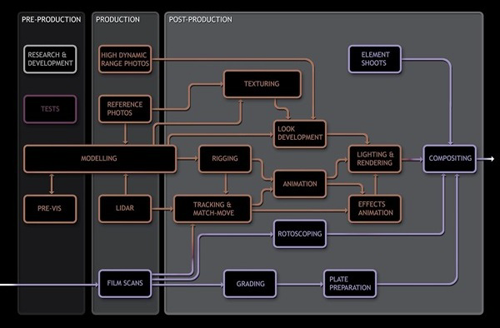
\includegraphics[width=0.8\textwidth,height=\textheight]{./images/andrew_whitehurst_pipeline.png}
\caption{An example pipeline (\emph{Andrew Whitehurst})}
\end{figure}

Collaboration between artists all working with different software packages and file formats introduces the need for a new area in companies large enough to afford them: the pipeline department. They are responsible for creating and managing custom infrastructures that aim to make interactions between different departments more efficient. With companies such as Double Negative and Cinesite branching into the world of feature animation, new and adventurous routes are being explored, with the ultimate goal of having the most cost-effective (efficient) and functional pipeline.

I explore the functions of all of the major creative departments you might find in a VFX house in Unit 10 (VFX Craft). So instead, here is a brief summary of what they each might output.


\pagebreak

\begin{longtable}[]{@{}ll@{}}
\toprule
Discipline & Output\tabularnewline
\midrule
\endhead
Onset & Reference photos, HDRIs, LIDAR/3D scans\tabularnewline
Concept & 2D \& 3D art\tabularnewline
Modelling & 3D models\tabularnewline
Rigging & Deformable character rigs\tabularnewline
Texture \& Shader Design & Texture maps, Shader scripts\tabularnewline
Environments/DMP & 3D geometry, Matte paintings\tabularnewline
Matchmove & 3D Cameras, Animation curves\tabularnewline
Animation & Animation curves, Geometry caches\tabularnewline
Creature & Geometry caches\tabularnewline
FX & Geometry caches\tabularnewline
Lighting & Light rigs, 2D passes\tabularnewline
Roto / Prep & 2D elements\tabularnewline
Comp & 2D sequences\tabularnewline
\bottomrule
\end{longtable}

\hypertarget{the-pipeline-tds-role}{%
\subsection{The Pipeline TD's Role}\label{the-pipeline-tds-role}}

Aside from the example above, a Pipeline TD also has many other responsibilities. I will explain a few below.

\emph{Note: By ``Pipeline TD'', I am making a generalisation and referring to members of the pipeline department, whose titles probably differ.}

\hypertarget{artist-workflow-tools}{%
\subsubsection{Artist Workflow Tools}\label{artist-workflow-tools}}

There may be some very specific tools that a show requires, or some general workflow tools that an application of choice doesn't do so well, that pipeline may be asked to develop.

\hypertarget{production-workflow-tools}{%
\subsubsection{Production Workflow Tools}\label{production-workflow-tools}}

In some cases, production may ask pipeline for specific tools to more easily meet their demands.

\hypertarget{meeting-production-demands}{%
\subsubsection{Meeting Production Demands}\label{meeting-production-demands}}

As in any business role, when faced with an issue, Pipeline TDs have to find a balance between the practical solution and the idyllic one. There can be pressure to complete a script, or push some renders through as soon as possible. The TD needs to have a good enough understanding of the production, creative, \& technical processes at the company to realise the impact that the decision might have on other projects or the studio.

\pagebreak\hypertarget{data-management}{%
\section{DATA MANAGEMENT}\label{data-management}}

Whether for streaming lossless 4k 32-bit EXRs or reading 500-gigabyte alembic caches, VFX studios require special and expensive infrastructure to enable working efficiently with such large amounts of data. They need to ensure that there is plenty of disk space for data, that there are reliable snapshot backup and archiving systems, that it is all accessible via a speedy network and that it is all protected by a hefty firewall.

\hypertarget{types-of-storage}{%
\subsection{Types of Storage}\label{types-of-storage}}

\hypertarget{online}{%
\subsubsection{Online}\label{online}}

This is data that is available to access instantaneously, over a network.

\hypertarget{nearline}{%
\subsubsection{Nearline}\label{nearline}}

Nearline storage is an intermediate between ``online'' and ``offline'' storage. It includes any data that is only online and available to access once it has been requested. It is much more power \& cost efficient for data to be nearline than online if it is not in constant use, as any disks that aren't currently in use don't have to be constantly spinning. A potential use might be for short-term backups.

\hypertarget{offline}{%
\subsubsection{Offline}\label{offline}}

Offline storage is any data not accessible from a network. This includes any storage on removable media (i.e.~USB flash drives, optical discs..) that is not currently connected or mounted on a computer and that would require some type of intervention to be available. Old or no longer immediately useful data is often archived and taken offline, as explained in the next section.

\hypertarget{backups-archiving}{%
\subsection{Backups / Archiving}\label{backups-archiving}}

Backups are copies of files that are safely stored for use in an event of the live data being lost, infected, or corrupted.

This is a vitally important risk-prevention measure for any modern company. In some cases losing data leads to lost money, from not only the cost of creating that data but also any costs of missing contracted deadlines not to mention the loss of a client's trust, which is perhaps more valuable. For example, in the context of VFX, a small 3mb Maya scene file would be very cheap to back up though, if it were corrupted, the loss could be a whole weeks work of a talented animator.

Snapshot systems are one method of backing up data. This is when changes to a machine's filesystem, called snapshots, are recorded and stored at regular intervals. Retention rules for the snapshots are set, to delete unwanted backups after a set period of time, to limit storage use. An example of how these could be set up: The system may retain one snapshot per hour for the last 24 hours, a snapshot per day for the past 7 days, a snapshot per week for the last 4 weeks, and a snapshot per month for the past 6 months. From this example, you can clearly see how any risk caused by accidental deletion or modification of files is greatly minimized, so long as the issue is spotted quickly.

\begin{figure}
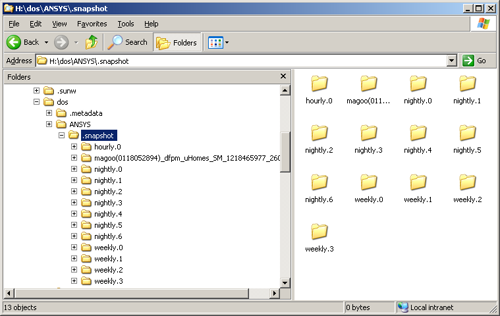
\includegraphics[width=0.6\textwidth,height=\textheight]{./images/snapshot_dirs.png}
\caption{Example snapshot directories}
\end{figure}

Archiving is another valuable data-protection measure. This is done when data that is not currently required is stored for the long-term. The main difference between a backup and an archive is that backups are created for live data, where it might be difficult or time-consuming to judge the importance or efficiency of protecting individual files, so they are protected indiscriminately, whereas the process of archiving is not always as time-critical, so files can be indexed and unnecessary data can be pruned.

It is common for WORM storage to be used for archiving data, which stands for ``Write Once, Read Many''. A well-known example of this type of storage is the CD-ROM. The advantage of WORM media is that it is protected from modification after it has been written so that data is protected for reference in the future. The most common medium used commercially today is the LTO (Linear Tape-Open) drive, which is a tape standard that is capable of storing a lot of data cheaply, relative to optical disks, on reels of hundreds of metres of several micrometre thick magnetic tape. The latest standard, LTO-8 (eighth generation) allows for tapes 12TB in capacity, and support write-protection and encryption.

\hypertarget{data-security}{%
\subsection{Data Security}\label{data-security}}

Data security covers measures that prevent unauthorized access to information. It is easy to understand why such measures are so incredibly important, to protect personal information such as communications, medical records, and bank details from destructive forces. In today's competitive world, virtually every successful company relies on the worth of privacy and security of sensitive data of all kinds. For example business plans, trade secrets, and private research. Our value of commercially-sensitive information is reflected in our legal systems by protecting laws and written contracts and holding people or corporate entities accountable by them.

\hypertarget{encryption}{%
\subsubsection{Encryption}\label{encryption}}

Encryption is one method used everywhere to keep our information secure. To encrypt data, it is put through a mathematical cryptographic algorithm which makes it unreadable to anyone without the right keys that may intercept it. These algorithms are in some way similar to common text cyphers where you might substitute certain characters with others, according to a key shared among the data's owners. However, cyphers for use with electronic data are millions of times more complex and could take hundreds of years to crack with current technology.

\pagebreak\hypertarget{render-management}{%
\section{RENDER MANAGEMENT}\label{render-management}}

Rendering high detail, photorealistic images and simulations calls for a lot of computer processing power. VFX houses need to be able to produce these results quickly. To do this, they often have their own in house super-computers, called render farms, which utilize the power of grid and cluster computing.

\hypertarget{what-is-grid-computing}{%
\subsection{What is Grid Computing?}\label{what-is-grid-computing}}

This describes a shared pool of computing resources used to solve complex tasks. It is a form of distributed computing, meaning that these tasks utilize the resources of multiple networked machine . In the context of visual effects, there are a number of examples where this can be used.

\hypertarget{security}{%
\subsubsection{Security}\label{security}}

In an industry that constantly deals commercially sensitive data, security is a huge priority. For larger studios, having workstations with access to internal servers and the internet can be risky territory as any breach of security due to malicious attacks would have direct access to this sensitive data. One solution to this that has been adopted by multiple studios it to use remote desktop environments provided by a server with internet access. This This adds a layer of protection, as any file transfers between a secure workstation and one of these remote environments is can be heavily controlled, which not only decreases the risk of a harmful malicious attack, but also acts as a deterrent against any leaks that might be caused internally.

There are many frameworks that utilize the efficiency of shared computing resources that enable for this type of remote environment. It would not be efficient to keep a virtual environment that isn't being used open, so after a session has been inactive for a period of time it is closed and resources are redistributed. Though it this isn't necessarily classed as grid computing as there is no distribution between networked machines involved.

\hypertarget{working-remotely}{%
\subsubsection{Working Remotely}\label{working-remotely}}

These virtual environments are used by many companies, and can be very cost-effective. Nvidia Grid is an example of a technology which enables this virtual desktop infrastructure (VDI) to be powerful to be practical for use in VFX production. Sharing resources over a number of Grid-enabled physical GPUs allows for a customised virtual GPU per user, making is possible to work in GPU intensive 3D programs without the need for multiple physical workstations.

\hypertarget{rendering}{%
\subsubsection{Rendering}\label{rendering}}

Many VFX studios, especially larger ones, have a number of powerful machines dedicated for rendering, which are called \emph{slaves}. Today, these can often be supplemented, or even fully replaced by, a number of remote machines provided by a cloud services such as YellowDog and Google Cloud. Pixar's Tractor is a system we use at DNEG that enables this distributed rendering. Tractor uses a central server and multiple render machines, called blades. It also provides a number of APIs and a web UI.

\hypertarget{understanding-tractor}{%
\subsubsection{Understanding Tractor}\label{understanding-tractor}}

Tractor blades can have multiple slots, and the number of slots describes the number of tasks a blade can run simultaneously. The central server, also called a queue manager, receives render jobs, containing a tree of individual tasks, which it distributes to available slots. These slots then run their specific tasks, which could be anything from a shell command which renames or moves a number of files to a 500 frame FX cache. After these tasks are completed, the blade will send a signal to the central server, announcing that it is ready for a new task.

Tasks can also be run on workstations, which are often abundant in a VFX studio. This is especially efficient at night, while these machines are not in use.

These tasks can also be given keys which are used by the queue manager to identify important information such as the application being used and the minimum specifications of the machine it can be run on. For example, a heavy lighting render may require a machine with a lot of RAM available and a powerful GPU, while a 2D prep nuke script can be rendered quickly on a machine with a much lower spec.

Job priority levels and limits can also be set too, which enable time-critical jobs to be run quickly while not taking too many slots from the rest of the farm. \texttt{priority} is a float attribute which is a measure of a jobs importance. The queue manager will allocate slots to tasks of higher priority jobs before lower priority jobs. Jobs in Tractor also have an attribute called \texttt{maxactive}, which defines the maximum number of active tasks available at one time. This would be useful in the case that a high priority job had 1000 tasks in parallel in their default state: \texttt{ready}. Without a max active set on the job, the queue manager would quickly allocate any available slots to this one job and would neglect any lower priority jobs.

\hypertarget{chunking}{%
\subparagraph{Chunking}\label{chunking}}

Chunking is when long sequences are split up into multiple tasks. This is a useful technique which speeds up jobs at the cost of CPUs. This is normally done by either splitting render sequences into smaller chunks of frames (e.g.~1 task per 10 frames), or by rendering different segments of an image as multiple tasks, for example splitting frames in half and rendering them as seperate tasks, before having a script stitch them back together. The latter is usually reserved for especially high resolution images, such as those for marketing stills.

\hypertarget{render-wrangling}{%
\subsubsection{Render Wrangling}\label{render-wrangling}}

\hypertarget{erroring-jobs}{%
\paragraph{Erroring Jobs}\label{erroring-jobs}}

One responsibility of a render wrangler (sometimes called a render TD) is to debug failing renders. Failing renders are easy to spot in tractor as the job is coloured bright red and reads ``error''. Any stack traces, errors or warnings should show in a tasks log, which can be access by right-clicking on a red errored task under the errored job in tractor, and selecting ``Log'' from the context menu. If the stack trace doesn't make much sense, there should be a scene file you can debug directly. First step would be to try and run the task manually step-by-step and see if you encounter any errors.

\hypertarget{slow-jobs}{%
\paragraph{Slow Jobs}\label{slow-jobs}}

There are many causes for slow or hanging jobs, and sometimes it can be difficult to diagnose a cause, especially when the log isn't showing any actual errors. Memory issues can often be the cause of hanging jobs, and the there are a few solutions for this. Namely:

\begin{itemize}
\tightlist
\item
  Retrying the issue on a slot with a higher RAM allocation.
\item
  Making the scene lighter. e.g.~rendering lower LODs of distant assets.
\item
  Chunking the job into smaller tasks.
\end{itemize}

For lighting renders, you can speed up the tasks by lowering the number of samples, which will result in a render being more noisy, though it can be quicker to render, then fix this noise using 2D tools than to render with a higher sample rate. In some cases, when the 2D noise removal is done well, these results can look very similar to a full-quality render.

\pagebreak\hypertarget{databases}{%
\section{DATABASES}\label{databases}}

\hypertarget{what-is-data}{%
\subsection{What is Data?}\label{what-is-data}}

Data describes any pieces of information. It can be split into two types:

\begin{itemize}
\item
  Structured Data \textgreater{}Structured data is data that is organised in a context with tags. A database is a collection of structured data.
\item
  Unstructured Data \textgreater{}Unstructured data is data with no context. This can be in the form of texts, images or any other forms of information.
\end{itemize}

\hypertarget{ensuring-quality-of-data.}{%
\subsection{Ensuring Quality of Data.}\label{ensuring-quality-of-data.}}

\hypertarget{validation}{%
\subsubsection{Validation}\label{validation}}

Validation is very important when inputting data into a database. It is the act of ensuring that data of the correct type and format is entered so that it can be sorted and understood, fitting in the correct context. For example, a list of dates of birth could be stored in a variety of ways but having one consistent format makes it much easier to order and query.

\begin{longtable}[]{@{}cc@{}}
\toprule
Validated & Not Validated\tabularnewline
\midrule
\endhead
\texttt{25.09.1998} & \texttt{25/009/98}\tabularnewline
\texttt{01.02.1965} & \texttt{2/1/65}\tabularnewline
\texttt{30.01.1989} & \texttt{06.1.89}\tabularnewline
\texttt{05.05.2005} & \texttt{5,\ 5,05}\tabularnewline
\bottomrule
\end{longtable}

\hypertarget{verification}{%
\subsubsection{Verification}\label{verification}}

Verification is another important practice that is used during data entry. It is to ensure that the correct data is being entered. Obviously, this could be slightly more difficult to check as the client that is being used to enter the data often isn't clever enough to know whether the data is correct, so verification is mostly used to correct human error. One method that is used is double entry: asking the user to enter the data twice.

A relational database consists of a series of tables of structured data. These tables are referenced using keys. The primary key is a unique id of a record in the current table, and the secondary key is that of a referenced table.

\hypertarget{relational-databases}{%
\subsection{Relational Databases}\label{relational-databases}}

Relational databases use multiple tables, and rows (also known as records) in a table refer to primary keys (unique-per-row values; normally a integer or hash) from other tables, enabling for complexity and efficiency that might not be possible in a traditional 2 dimensional database.

Different tables are usually created for different ``object types''. For example, in the context of VFX, there might be a table for shots, a table for assets and a table for asset versions. The assets table might include a number of different items that are being worked on for a specific shot. These assets would have a reference to the shot that they belong to's primary key from the shot table.

\hypertarget{querying-a-database}{%
\subsubsection{Querying a Database}\label{querying-a-database}}

At DNEG I have written a number of tools which use queries read information from our database and our shotgun database. The tools I have used to interact with both of these are APIs, which add a layer of abstraction and make querying much more user friendly, and also much less dangerous. Deleting and editing data is much more protected than it would be interacting directly with the MySQL and PostgreSQL servers.

This shotgun query returns a list of dictionaries containing the \texttt{name} attribute of all projects in the shotgun database whose \texttt{sg\_status} attribute is ``active''.

\begin{verbatim}
from shotgun.common import conn
active_shows = conn.shn.find(
    "Project",
    [["sg_status","is","Active"]],
    fields = ["name", "sg_status"]
)
[
    {
        'sg_status': 'Active',
        'type': 'Project',
        'id': 4,
        'name': 'DNEG_SHOW1'
    },
    {
        'sg_status': 'Active',
        'type': 'Project',
        'id': 67,
        'name': 'DNEG_SHOW2'
    },
    # etc...
]
\end{verbatim}

\pagebreak\hypertarget{project-organisation}{%
\section{PROJECT ORGANISATION}\label{project-organisation}}

\hypertarget{vfx-production}{%
\subsection{VFX Production}\label{vfx-production}}

Large-scale VFX projects may require collaboration between hundreds of different people over several different sites globally, which is the reason that production teams exist. Production holds the responsibility of managing artists, liaising with clients and creating \& maintaining realistic work schedules, among other things.

One system that is popular among many VFX studios is \emph{Shotgun}. Shotgun is primarily a project management system designed specifically for animation and VFX production, which includes an integrated asset management and versioning system. It's used by artists and production alike, with one of its major selling points being its all-in-one approach; Production can use it to easily set team milestones and distribute tasks, while artists can use it to keep track of their work and respond to all their latest notes.

\begin{figure}
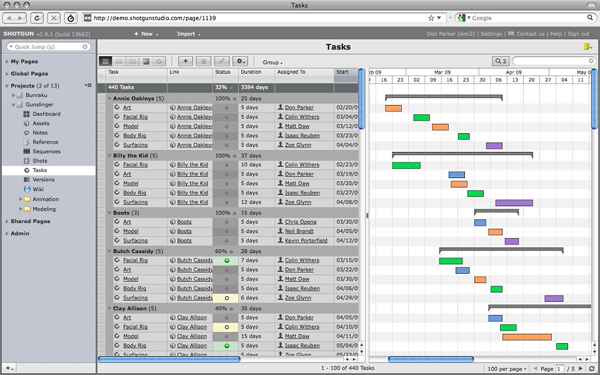
\includegraphics[width=0.8\textwidth,height=\textheight]{./images/shotgun_task_view.png}
\caption{Shotgun's web interface}
\end{figure}

\hypertarget{version-control}{%
\subsubsection{Version Control}\label{version-control}}

An effective way to track the progress of something being developed is by using version control. This applies not only to the artist side for digital assets but to software packages and scripts also. In its simplest form, this means saving your work into at sensible intervals and keeping a history of your previous work. This is useful for creative development as it allows an artist or a supervisor to look at the development of an asset to ensure that it is heading in the right direction. Shotgun has a version control system built in and is packaged with the review software RV, which allows you to compare and annotate different iterations of an artist's work.

On the technical side, this method allows you to look at the history of a tool to help spot or prevent issues that in the development of it. Package management systems are often used for deploying tools and scripts to studios, which almost always will include its own versioning system. \emph{As explained in Unit 8, Git is also very commonly used as well, as a version control system for of source code. The difference being that package management systems will version an entire package on build, while Git manages all code changes on any number files within the package, between and including package version iterations.}

\hypertarget{pluginsoftware-production}{%
\subsection{Plugin/software Production}\label{pluginsoftware-production}}

While the idea of an all-in-one pipeline solution sounds great, there is always room for development to meet the ever-changing demands of clients and to best suit the studio. For instance, often different clients will use different naming conventions they wish you to follow. Some studios have technical developers crewed to shows, who create and maintain custom tools to aid production. \emph{Further explained in unit 1.}

\pagebreak\hypertarget{maths}{%
\section{MATHS}\label{maths}}

\hypertarget{basic-algebra}{%
\subsection{Basic Algebra}\label{basic-algebra}}

Under this very broad subheading, I will give some examples of how to rearrange mathematical statements, that you can use to simplify expressions and solve equations for unknowns.

\hypertarget{simplifying}{%
\subsubsection{Simplifying}\label{simplifying}}

We can collect like terms in equations to make them simpler to express.

\[4x+2y-8x+y\]

Here, 2 terms, \(4x\) and \(-8x\), are a product of \(x\). Together they are equal to \((4-8)x=-4x\). If we do the same for the y terms and take the sum the result we get a totally simplified expression, \(3y-4x\).

\[\frac{4x}{y}+\frac{3x}{2}-\frac{2y}{2}+2x\]

Here we can have 3 factor that we cannot simplify, \(x\), \(y\) and \(x/y\). Using the same method as above, we take the 2 \(x\) terms and substitute them for their the sum of the two.

\[\frac{3x}{2}+2x=\frac{3x}{2}+\frac{4x}{2}=\frac{7x}{2}\]

Now to simplify \(2y/2\):

\[\frac{2y}{2}=\frac{2}{2}\times y=1 \times y = y\]

So, the simplified expression:

\[\frac{4x}{y}+\frac{7x}{2}-y\]

\hypertarget{rearranging-equations}{%
\subsubsection{Rearranging Equations}\label{rearranging-equations}}

An equation is a statement in which two mathematical expressions are equal to each other. There is really just one rule that, so long as it is followed, makes rearranging equations simple.

\begin{quote}
You can perform mathematical operations on each ``side'' of the equation, so long as you perform equal operations to all sides.
\end{quote}

Let's start with this example:

\[x+\sqrt{4y}=5+x\]

Here, if we wanted to solve for \(y\), we could subtract \(x\) from each side and we are left with \(\sqrt{4y}=5\). Next, we need to get rid of the square root. We can do this by taking a square of both sides. This involves multiplying both sides of the equation with an equal expression, so it still very much follows our one rule. After simplifying \(\sqrt{4y}^2=5^2\), we have \(4y=25\). Lastly, we can divide all sides by 4, which would leave us with \(y=25/4=6.25\).

This was a simple example but the same methodology is used when solving more complex equations such as polynomials. However, unknowns in many equations cannot be described by a single value and instead are being described as an expression which describes a range of possible values. You can craft equations with these which define shapes and curves.

\hypertarget{the-quadratic-equation}{%
\paragraph{The Quadratic Equation}\label{the-quadratic-equation}}

\[x=\frac{-b\pm\sqrt{b^2-4ac}}{2a}\]

Where:

\[ax^2+bx+c=0\]

When solving quadratics, this equation can be used to solve for \(x\). The \(\pm\) symbol means that the equation is true for both a \(+\) and a \(-\), as most quadratics have 2 solutions.

\hypertarget{trigonometry}{%
\subsection{Trigonometry}\label{trigonometry}}

Trigonometry encompasses the studies of ratios including side lengths and angles of triangles. I will cover how to solve a triangle side or angle using trigonometry.

\begin{figure}
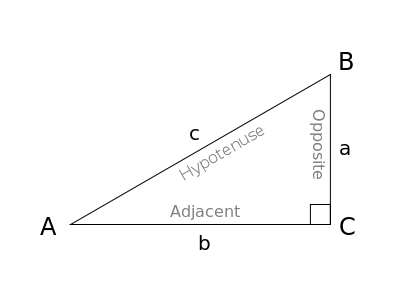
\includegraphics[width=0.7\textwidth,height=\textheight]{./images/trig_triangle.png}
\caption{Labeled triangle}
\end{figure}

There are two trig equations we will be using: the Sine rule and Pythagoras's equation.

\hypertarget{pythagoras-theorem}{%
\subsubsection{Pythagoras' Theorem}\label{pythagoras-theorem}}

Pythagoras' theorem states that with a triangle with sides labelled \(a\), \(b\) and \(c\), where \(c\) is that triangles hypotenuse:

\[a^2+b^2=c^2\]

We can use Pythagoras' theorem to calculate the length of a side of a triangle if we have the lengths of the 2 other sides. Let's try it in practice:

\begin{quote}
I have a triangle whose opposite side is 13cm, whose hypotenuse is 21cm and whose adjacent side is \(x\)cm. Calculate \(x\).
\end{quote}

So we can substitute 13cm and 21cm for \(a\) (\(b\) would be equally as valid) and \(c\) respectively. We now have:

\[13^2\mathrm{cm}+b^2=21^2\mathrm{cm}\]

If we subtract \(13^2\mathrm{cm}\), we get \(b^2=21^2\mathrm{cm}-13^2\mathrm{cm}\). Next step is to take the square root of each side, and evaluate:

\[b=\sqrt{21^2\mathrm{cm}-13^2\mathrm{cm}}=16.492\]

\hypertarget{the-sine-rule}{%
\subsubsection{The Sine Rule}\label{the-sine-rule}}

\[\frac{sin(A)}{a}=\frac{sin(B)}{b}=\frac{sin(C)}{c}\]

We can use the rule to calculate lengths and angles of any triangle. (\(a\), \(A\)), (\(b\), \(B\)) and (\(c\), \(C\)) refer to length and angle pairs opposite each other, as displayed in the diagram earlier in this section.

Let's use this rule to solve for x in this triangle.

\begin{figure}

\includegraphics[width=0.7\textwidth,height=\textheight]{./images/trig_triangle_2.png}
\caption{Incomplete triangle}
\end{figure}

\hypertarget{substituting-known-values}{%
\paragraph{Substituting known values}\label{substituting-known-values}}

The first step is to substitute our known values into this rule. It is useful to note that \(sin(90)=1\).

\[\frac{1}{15\mathrm{cm}}=\frac{sin(38 )}{x\mathrm{cm}}\]

\hypertarget{taking-the-reciprocal}{%
\paragraph{Taking the reciprocal}\label{taking-the-reciprocal}}

Next, we can take the reciprocal (flip the fraction) of each side. This still fits our one rule as it is the same as raising the expression on each side by a power of \(-1\).

i.e. \textgreater{}\(x^{-1}=\frac{1}{x}\) \textgreater{} \textgreater{}\(\frac{4}{x}^{-1}=\frac{1}{x}\times4=\frac{4}{x}\)

\hypertarget{move-known-terms-to-one-side}{%
\paragraph{Move known terms to one side}\label{move-known-terms-to-one-side}}

\[15\mathrm{cm}=\frac{x\mathrm{cm}}{sin(38)}\]

We can do this by multiplying each side by \(sin(38)\), leaving us with a single expression, \(15sin(38)\), which, when evaluated, is equal to \(x\).

\[15sin(38)=x\mathrm{cm}=9.235\mathrm{cm}\]

\hypertarget{using-the-inverse-sine-function}{%
\paragraph{Using the inverse sine function}\label{using-the-inverse-sine-function}}

When solving for an angle using the sine rule you are left with an unknown in the sine function, after using the standard operators. Here is an example:

\[\frac{sin(90)}{5}=\frac{sin(x)}{4}\] \[\frac{4}{5}=sin(x)\]

Here we can use the inverse sin function (\(sin^{-1}()\)) to solve for x:

\[sin^{-1}\left(\frac{4}{5}\right)=53.130\]

\hypertarget{vectors}{%
\subsection{Vectors}\label{vectors}}

A vector is a quantity with more than 1 dimension. It has both a direction and a magnitude. In 2D space, we can use vectors to describe the difference between 2 points. For example, if we had 2 points, \(a(13.6,\space4.2)\) and \(b(-3,\space1.1)\), we could find the vector between them by finding the difference between the \(x\) and \(y\) components of the points. We can describe the vector from \(a\) to \(b\) as \(\vec{ab}\).

\[\vec{ab}=\begin{pmatrix}
-3-13.6\\1.1-4.2
\end{pmatrix}=
\begin{pmatrix}
+16.6\\-3.1
\end{pmatrix}\]

We can now manipulate this vector the similarly to how we would scalar quantities (one-dimensional quantities).

Adding and subtracting vectors is easy. Let me show you an algebraic example with my two 3-dimensional vectors: \(\vec{p}\) and \(\vec{q}\)

\[
\vec{p}=\begin{pmatrix}
x_{1}\\y_{1}\\z_{1}
\end{pmatrix},\space
\vec{q}=\begin{pmatrix}
x_{2}\\y_{2}\\z_{2}
\end{pmatrix}
\] \[
\vec{p}+\vec{q}=\begin{pmatrix}
x_{1}+x_{2}\\y_{1}+y_{2}\\z_{1}+z_{2}
\end{pmatrix},\space\vec{p}-\vec{q}=\begin{pmatrix}
x_{1}-x_{2}\\y_{1}-y_{2}\\z_{1}-z_{2}
\end{pmatrix}
\]

\hypertarget{matrices}{%
\subsection{Matrices}\label{matrices}}

\hypertarget{addition}{%
\subsubsection{Addition}\label{addition}}

Adding and subtracting matrices from other matrices is only possible for matrices with the same dimensions. Here we will add two 2 by 2 matrices together. It is as simple as just finding the sum of each corresponding value.

\[\begin{pmatrix}3&7\\-9&8\end{pmatrix}+\begin{pmatrix}-1&-3\\5&6\end{pmatrix}=\begin{pmatrix}3-1&7-3\\-9+5&8+6\end{pmatrix}=\begin{pmatrix}2&4\\-4&14\end{pmatrix}\]

\hypertarget{multiplication}{%
\subsubsection{Multiplication}\label{multiplication}}

Multiplication is a little more difficult. The number of rows in matrix 1 must match the number of columns in the second matrix. You solve them each row/column pair at a time.

\[\begin{pmatrix}4&2&-1\\3&-5&2\\\end{pmatrix}\times
\begin{pmatrix}2&6\\1&8\\1&2\end{pmatrix}=\] \[
\begin{pmatrix}
    \begin{pmatrix}4&2&-1\end{pmatrix}\times
    \begin{pmatrix}2\\1\\1\end{pmatrix}
&
    \begin{pmatrix}4&2&-1\end{pmatrix}\times
    \begin{pmatrix}6\\8\\2\end{pmatrix}
\\
    \begin{pmatrix}3&-5&2\end{pmatrix}\times
    \begin{pmatrix}2\\1\\1\end{pmatrix}
&
    \begin{pmatrix}3&-5&2\end{pmatrix}\times
    \begin{pmatrix}6\\8\\2\end{pmatrix}
&\end{pmatrix}
\]

Let's first try to solve the first value of our new matrix. To do this we need to know how to multiply a row by a column. We just multiply each value, starting from the left of the row, to its corresponding value in the column, counting starting from the top.

\[\begin{pmatrix}4&2&-1\end{pmatrix}\times
\begin{pmatrix}2\\1\\1\end{pmatrix}=
(4\times2)+(2\times1)+(-1\times1)=9\]

Now we just do that for each other row \& column pair, and then we have our result.

\[\begin{pmatrix}4&2&-1\end{pmatrix}\times
\begin{pmatrix}6\\8\\2\end{pmatrix}=
(4\times6)+(2\times8)+(-1\times2)=38\]

\[\begin{pmatrix}3&-5&2\end{pmatrix}\times
\begin{pmatrix}2\\1\\1\end{pmatrix}=
(3\times2)+(-5\times1)+(2\times1)=3\]

\[\begin{pmatrix}3&-5&2\end{pmatrix}\times\begin{pmatrix}6\\8\\2\end{pmatrix}=(3\times6)+(-5\times8)+(2\times2)=-18\]

\hypertarget{the-result}{%
\paragraph{The result:}\label{the-result}}

\[\begin{pmatrix}4&2&-1\\3&-5&2\\\end{pmatrix}\times
\begin{pmatrix}2&6\\1&8\\1&2\end{pmatrix}=\begin{pmatrix}9&38\\3&-18\end{pmatrix}\]

\hypertarget{mechanics}{%
\subsection{Mechanics}\label{mechanics}}

\hypertarget{equations-of-motion}{%
\subsubsection{Equations of motion}\label{equations-of-motion}}

\begin{longtable}[]{@{}l@{}}
\toprule
SUVAT equations\tabularnewline
\midrule
\endhead
\(v=at+u\)\tabularnewline
\(s=ut+\frac{1}{2}at^2\)\tabularnewline
\(s=\frac{1}{2}(v+u)t\)\tabularnewline
\(v^2=u^2+2as\)\tabularnewline
\bottomrule
\end{longtable}

These equations of motion, usually called SUVAT equations, can be used to model motion under constant acceleration. The letters \(s\), \(u\), \(v\), \(a\) \& \(t\) are used to form these equations (hence SUVAT). This is what each letter means:

\begin{itemize}
\tightlist
\item
  \textbf{s}: Displacement.
\item
  \textbf{u}: Initial velocity.
\item
  \textbf{v}: Final velocity.
\item
  \textbf{a}: Acceleration.
\item
  \textbf{t}: Time.
\end{itemize}

If we have a scenario in which we have a number of these elements, we can substitute them into one of these equations in an attempt to solve an unknown. For example, take this problem:

\begin{quote}
A man throws a football, which leaves his hand at .3m/s, 140cm from the ground. Assuming that his hand was in line with his front foot as the ball left his hand, how far from the man is the position of the ball as it first touches the ground?
\end{quote}

Assuming that the force of gravity on his planet is equal to \(-9.81\mathrm{m/s}^2\), here is the information we know, for each component in \(x\) and \(y\).

\(x\) component

\begin{itemize}
\tightlist
\item
  \(s_{x}=\) ? (What we need to find)
\item
  \(u_{x}=\) \(0.3\mathrm{m/s}\)
\item
  \(v_{x}=\) \(0.3\mathrm{m/s}\)
\item
  \(a_{x}=\) \(0\mathrm{m/s}^2\)
\item
  \(t=\) ?
\end{itemize}

\(y\) component

\begin{itemize}
\tightlist
\item
  \(s_{y}=\) \(1.4\mathrm{m}\)
\item
  \(u_{y}=\) \(0\mathrm{m/s}\)
\item
  \(v_{y}=\) ?
\item
  \(a_{y}=\) \(-9.81\mathrm{m/s}^2\)
\item
  \(t=\) ?
\end{itemize}

If we solve for the time (\(t\)) using the y component, we can then use it to find \(s_{x}\). We can use the second equation for this: \(s=ut+\frac{1}{2}at^2\). First let's rearrange for \(t\).

First we will multiply each side by 2, for nicer numbers: \[2s=2u_{y}t+a_{y}t^2\]

Then we can subtract \(2s_{y}\) from each side, to create a quadratic: \[a_{y}t^2+2u_{y}t-2s_{y}=0\]

Then solve for \(t\) using the quadratic equation:

\begin{quote}
\[x=\frac{-b\pm\sqrt{b^2-4ac}}{2a}\]
\end{quote}

\[a=a_{y},\space b=2u_{y},\space c=2s_{y}\]

\[t=\frac{-2u_{y}\pm\sqrt{2u_{y}^2-4a_{y}2s_{y}}}{2a_{y}}\]

Now we can substitute in our values: \[t=\frac{-0\pm\sqrt{0^2-4(-9.81)(2*1.4)}}{2(-9.81)}\] And simplify: \[t=\frac{\pm\sqrt{-4(-9.81)(2.8)}}{2(-9.81)}=
\frac{\pm\sqrt{109.872}}{-19.62}=\pm0.534\]

We'll discard the negative value as it doesn't really make sense in our scenario. Now we know how long it took for the ball to hit the floor (\(t\)). We can use it to solve for \(s_{x}\) and find the solution to this problem. This next equation seems right for solving the x component:

\[s=\frac{1}{2}(v+u)t\]

We just need to substitute in our values:

\[s_{x}=\frac{1}{2}(0.3\mathrm{m/s}+0.3\mathrm{m/s})\times0.534\mathrm{m}=0.3\mathrm{m/s}\times0.534\mathrm{m}\] \[s_{x}=0.160\mathrm{m}=16\mathrm{cm}\]

And there is our result. Clearly, he isn't a very good throw.

Mechanics are important in everyday work for many visual effects artists, namely artists in the FX department. Something that makes digital performances seem so believable on screen is the way objects move and are interacted with in a physically realistic way. Simulations of particles, fluids, cloth, hair and others are all based on how dynamics in the real world behave. This was just a very basic example.

\pagebreak\hypertarget{software-design}{%
\section{SOFTWARE DESIGN}\label{software-design}}

Software Design is the process of creating a detailed schematic of a piece of software that meets the requirements of a given brief. This could be a for building upon a piece of existing software, or an entirely new project.

\hypertarget{choosing-a-language}{%
\subsection{Choosing a Language}\label{choosing-a-language}}

If a new piece of software is being designed, there are many different programming languages that you could decide to build it with, each offering different advantages. A good rule of thumb is that the lower the level of language used (The less abstract languages), the more efficient your software can be. For example, you could probably write a relatively fast program in C. But using a higher level language such as C++, Pascal, or Java might mean that the software will be finished faster, as they tend to be faster to write in. Interpreted scripting languages such as Python may also be an option, as the development and support work can happen quickly. Speed and fluidity is not always the number one concern.

\hypertarget{pseudocode}{%
\subsection{Pseudocode}\label{pseudocode}}

Pseudocode is a notation that describes the step-by-step logic behind a particular algorithm, that is used in the planning stage of software development. There is no universal format, so it is subjective and informal. The primary aim of it is to be readable and understandable to other developers who might read it.

It is often used as an intermediate between the planning stage and writing functional code. Here is an example of a function that returns the factorial of given value, in pseudocode.

\begin{verbatim}
FUNCTION get_factorial(value)
    factorial = 1
    FOR i in all integers from 1 to i >= value
        factorial = factorial * i

    WRITE "Factorial of "+ value +" = " + factorial
    RETURN factorial
\end{verbatim}

\hypertarget{testing}{%
\subsection{Testing}\label{testing}}

Testing is an important method used for minimizing the risk of damage caused by a new release of a piece of software. Unit tests are scripts specific to a piece of software that are often run upon a new build. Given known input and output pairs of functions in the software, these tests will ensure that functions in this build give correct outputs, and when given invalid inputs, they error correctly.

Integration tests are scripts that ensure that different components or modules work correctly together. These are important because of two reasons: Because unit tests often can't cover every possibility, and because unit tests only test within in either a single module or selection of modules. Though other modules from outside that scope might depend on functions from within it, so if any behaviour were to change, then these modules should be tested too.

\hypertarget{version-control-1}{%
\subsection{Version Control}\label{version-control-1}}

The development of software is never a linear process. Often initial decisions on how a tool should work, or what a UI should look like are superceded either feedback from testers or clients, or by unforeseen technical limitations or capabilities. Code is constantly being modified, removed, and overwritten. This is one reason why tracking development work is critical. It is very cheap to backup old versions of scripts and libraries as are just text files, yet the cost of the time of the developer can be very expensive.

There are a wide variety of solutions available to manage development and version but I will cover two that are commonly used.

\hypertarget{package-management-systems}{%
\subsubsection{Package-Management Systems}\label{package-management-systems}}

Package management systems are often used for building and deploying tools and scripts. These are often centralized systems which store information about builds of software. Examples of what this information might include are the creator of the build, the time it was built, the compiled build files and information about any dependencies of the software.

\hypertarget{git}{%
\subsubsection{Git}\label{git}}

Git is a distributed version control system (DVCS) that is used to manage source code development. ``Distributed'' means that there is no centralized server required. A Git repository is created for each project, which is a Git-managed directory in which source code for that project is stored. I will explain all of the main concepts that are essential for working with Git, and then go through the git commands you will most likely be using if you were using a Git workflow.

\hypertarget{commits}{%
\paragraph{Commits}\label{commits}}

Each developer ``commits'' his development work to Git and Git saves snapshot changes of source code. Over time, this effectively builds long chains of commits that describe modifications, additions and removals of files, an entire history of the source code, from the creation the repository to its current state.

\hypertarget{tags}{%
\paragraph{Tags}\label{tags}}

Tags are pointers to specific commits, which are often used to denote which commit a version was built from. These can be useful when debugging a particular build of the software. Tags are immutable, meaning that they cannot be overwritten, though they can be explicitly removed and a new tag re-added.

\hypertarget{branches}{%
\paragraph{Branches}\label{branches}}

Git also features branching, a way to divide streams of development by the feature being worked on. These branches can then be merged into the source branch after these have been tested and reviewed. The most common way this is utilized is by having a primary branch, normally named \emph{master} or \emph{release}, which contains reviewed and tested code. Most in-use and/or released software will be built have been from this branch. But before feature branches are merged into this primary branch, there is normally an intermediate step, in which some reviewing and testing may take place. A secondary branch, which might be called \emph{develop} or \emph{testing}, is normally used as this step.

Branches are technically pointers to commits, in the same way as tags. What makes branches different is a branch's commit will update as you add/remove commits, while a tag will remain on a specific commit.

\hypertarget{head}{%
\paragraph{HEAD}\label{head}}

HEAD is a special pointer, which points to the commit you are currently working from. All of the files in your repository are a result of all parent commits up to HEAD, therefore HEAD can be thought of as the parent of your next commit. In most cases, it will point the branch you are working on, though there are some cases in which HEAD might not point to a branch's commit. This is called a detached HEAD.

\hypertarget{upstream-downstream-repositories}{%
\paragraph{Upstream \& Downstream Repositories}\label{upstream-downstream-repositories}}

A Git repository can be developed upon remotely, by multiple people, with no need for any centralized servers. The first step to working on a remote repository is by using a process called cloning. Cloning a repository copies the commits from the remote Git directory and configures the remote directory as an upstream repository. By default, this upstream will be named \texttt{origin}. The resultant, local repository is then known as a downstream. New commits and tags on the remote can be pulled on demand, and local changes can be pushed to the remote.

While I mentioned above that Git was a Distributed system, and that there is no need for a centralized server, many workflows do use a centralized server for holding repositories, which developers pull from and push to.

\hypertarget{working-with-git}{%
\subsubsection{Working with Git}\label{working-with-git}}

All of the text in these documents that you're reading are stored in Git-controlled markdown files. I show the processes of how contributing to Git projects works using this repository as an example.

\hypertarget{cloning}{%
\paragraph{Cloning}\label{cloning}}

The first step is to clone a remote repository that you wish to work on. This can be done using the \texttt{git\ clone} command and a path or URL to the remote repository.

\begin{verbatim}
>>> git clone https://github.com/HBalable/atd-apprentice-module-
summaries.git
Cloning into 'atd-apprentice-module-summaries'...
remote: Counting objects: 248, done.
remote: Compressing objects: 100% (93/93), done.
remote: Total 248 (delta 53), reused 12 (delta 3), pack-reused 150
Receiving objects: 100% (248/248), 3.56 MiB | 238.00 KiB/s, done.
Resolving deltas: 100% (123/123), done.
>>> cd ./atd-apprentice-module-summaries
\end{verbatim}

\texttt{git\ status} is a very useful command which shows information about your working tree, which is the current state of the source code in your local directory. We should see nothing much here, as we have not yet edited any of the files.

\begin{verbatim}
>>> git status
On branch master
Your branch is up to date with 'origin/master'.

nothing to commit, working tree clean
\end{verbatim}

We will want to create and switch to a new branch for our changes. We can create a new branch from the current branch (\texttt{master}) with the \texttt{git\ branch} command and we'll use the \texttt{git\ checkout} command to switch to it. Let's make a new branch called \texttt{example} and check it out.

\begin{verbatim}
>>> git branch example
>>> git checkout example
Switched to branch 'example'
\end{verbatim}

Now let's add a new file to the repository and see what happens.


\pagebreak

\begin{verbatim}
>>> touch example_file
>>> git status 
On branch example
Untracked files:
  (use "git add <file>..." to include in what will be committed)

        example_file

nothing added to commit but untracked files present (use "git add" 
to track)
\end{verbatim}

You can see that is prompting us to add this file using \texttt{git\ add} to stage it for commit. This extra step is useful for when you might want to commit different changes to different files separately. You only stage the files you want to be committed. Let's stage our file now.

\begin{verbatim}
>>> git add example_file
>>> git status
On branch example
Changes to be committed:
  (use "git reset HEAD <file>..." to unstage)

        new file:   example_file
\end{verbatim}

This file is now staged and ready to be committed. We now just need to use \texttt{git\ commit} command to commit it. We'll use the \texttt{-m} argument to pass a commit message too. These messages should be short sentences that summarise the changes in the commit.

\begin{verbatim}
>>> git commit -m "added example_file"
[example 97587c8] added example_file
 1 file changed, 0 insertions(+), 0 dele
\end{verbatim}

Now we've successfully committed our changes, we can merge them back into the source branch, using the \texttt{git\ merge} command. When working collaboratively on a project, you should never merge to master without at least some testing or reviewing of your code, but I will do it now, just as an example. To do this, we will first have to switch to the \texttt{master} branch.

\begin{verbatim}
>>> git checkout master
>>> git merge example
Updating 6a6fc51..97587c8
Fast-forward
 example_file | 0
 1 file changed, 0 insertions(+), 0 deletions(-)
 create mode 100644 example_file
\end{verbatim}

Now, we just need to push our branches back to the upstream repository, \texttt{origin}. We can do that using the \texttt{git\ push} command.


\pagebreak

\begin{verbatim}
>>> git push origin example
Total 0 (delta 0), reused 0 (delta 0)
https://github.com/HBalable/atd-apprentice-module-summaries.git
   6a6fc51..97587c8  example -> example  

>>> git push origin master
Counting objects: 2, done.
Delta compression using up to 4 threads.
Compressing objects: 100% (2/2), done.
Writing objects: 100% (2/2), 255 bytes | 255.00 KiB/s, done.
Total 2 (delta 0), reused 0 (delta 0)
To https://github.com/HBalable/atd-apprentice-module-summaries.git
   6a6fc51..97587c8  master -> master
\end{verbatim}

And that is how you successfully use Git for development, in it's simplest form. It is worth mentioning that \texttt{git\ init} is the command used for creating a brand new git repository from the current directory if you are not working from a remote. There are many other commands that prove to be useful, and plenty of information about them is accessible from the \texttt{git\ -\/-help} command.

\pagebreak\hypertarget{scripting}{%
\section{SCRIPTING}\label{scripting}}

\hypertarget{shell-scripting}{%
\subsection{Shell Scripting}\label{shell-scripting}}

Firstly, a shell describes something used to interface with an operating systems services, GUIs (Graphical User Interfaces) or CLI's (Command-Line Interfaces) are examples, though in this unit we will be focusing specifically on Command-line shells. On UNIX or Linux any command-line interpreters are called shells.

A shell script is a text file containing a set of instructions to be interpreted by a shell. This file can then be executed from a shell, which is much faster than doing all of these individual steps separately. These files can also be executed with arguments too like regular CLI commands. Most repetitive or menial tasks that can be done on a computer can be automated with scripts. For example, if you wanted to recursively trawl your hard drive and create an index of your files and how much space they took up, you could script it! Or say you wanted to get an update on the weather or the news when you opened your shell. You could script this too! Computers are great!

\hypertarget{the-hashbang}{%
\subsubsection{The Hashbang}\label{the-hashbang}}

In Linux or Unix, all shell scripts are expected to have a special first line, starting with what is called a hashbang (also called a she-bang), which looks like this \texttt{\#!}. This line tells the shell being used which interpreter should be used to execute the file.

For example tcsh..

\begin{verbatim}
#!/bin/tcsh
echo "Hello World!"
\end{verbatim}

Or Python\ldots{}

\begin{verbatim}
#!/usr/bin/env python2.7
print "Hallo Welt!"
\end{verbatim}

\hypertarget{python}{%
\subsection{Python}\label{python}}

Python is an interpreted programming language, which means that it doesn't need to be compiled into machine code before it is run, as opposed to compiled programming languages. One advantage of it is that it reads very similar to pseudocode (explained in module 7), which makes it fairly easy to understand at a glance.

\hypertarget{comparision-with-c}{%
\subsubsection{Comparision with C++}\label{comparision-with-c}}

Let me show you an example, I will define two identical functions: One in C++ and then one in Python,

\hypertarget{c-implemenation}{%
\paragraph{C++ Implemenation}\label{c-implemenation}}

\begin{verbatim}
int get_factorial(int value)
{
    int factorial=1;
    for (int i = 1; i <= value; ++i) {
        factorial *= i;
    }

    cout<< "Factorial of "<<value<<" = "<<factorial;
    return factorial;
}
\end{verbatim}

\hypertarget{python-equivilent}{%
\paragraph{Python Equivilent}\label{python-equivilent}}

\begin{verbatim}
def get_factorial(value):
    factorial = 1
    for i in xrange(1, value + 1):
        factorial *= i

    print("Factorial of {0} = {1}".format(value, factorial))
    return factorial
\end{verbatim}

At least for me, this second function is much easier to make sense of. There is much less punctuation used in the formatting of Python, which is something that can make C++ look quite confusing at first. One way Python achieves this is by requiring strict use of whitespace. You can see that the indentation quite consistent between the two functions, but the difference is that in Python this is required. We could remove this indentation in C++ and our function would compile and run just fine. For example, as horrible as it looks, here is a how our C++ function could have looked:

\begin{verbatim}
int get_factorial(int value){int factorial=
1;for(int i=1;i<=value;++i){factorial
*=i;}cout<<"Factorial of "<< value<<" = "<<
factorial;return factorial;}
\end{verbatim}

This works exactly as before, whereas straying too far from the formatting of our Python function gives us an error:


\pagebreak

\begin{verbatim}
>>> def get_factorial(value):
... factorial=1
  File "<stdin>", line 2
    factorial = 1
            ^
IndentationError: expected an indented block
\end{verbatim}

This is possible in C++ because it uses curly braces \texttt{\{\}} to contain code within constructs such as functions and for/while loops, and semicolons \texttt{;} to signify line endings (\emph{semicolons for line endings are supported in python syntax, but not encouraged unless required.}). The advantage of this strict whitespace formatting is that it encourages clear and easy to read code. This is one example of how using Python makes for code that is quick to understand and modify.

Another characteristic is that is that you do not need to declare variables until you use them, or set their type, which makes Python a \emph{dynamically-typed language}. Also, the language is entirely object-oriented, including every variable, therefore different types are just instances of different classes.

Though there is a cost to this freedom that comes with Python coding: execution speed. Given the right task, C++ could outperform Python more than 400 times over. But this is very understandable. This analogy might help:

\begin{quote}
Imagine having 2 guests over on a Friday evening for dinner. Guest 1's favourite food is ham/pineapple pizza, so you prepare him some. But you have never met guest 2 before, so you aren't sure what he likes, so you decide to buy a couple other pizza's that he might be into, including separate vegan and vegetarian options, just in case. Guest 1 is the C++ code, the compiler knows exactly what to expect and can prepare for it, and even perform some validation checks to help ensure everything will run smoothly and fast. Guest 2 on the other hand, is the python code. The objects being manipulated could be anything, so most validation would be useless. The interpreter relies on you writing working code.
\end{quote}

It's important to note that the Python interpreter is in fact written in C, a very popular statically-typed compiled language. C is compiled directly into machine code, which is perhaps the lowest level programming language: binary, which is executed directly by the CPU. It's also worth mentioning that interpreted languages are not necessarily slower than compiled languages. ASM (assembly language) is an interpreted language that can in many cases run tasks faster than compiled C, in fact, C was written in assembly language.

Though it may not be as speedy as other languages, Python is very effective in other areas. High-level abstraction and it's dynamically typed nature, make it a very easy language to learn and use, even for people who might not have programmed before. It is also much faster to write than a C program would be, as you don't have to spend so much time on memory-management and many useful algorithms and functions are already defined in the standard libraries.

\hypertarget{python-wrapped-apis}{%
\subsubsection{Python Wrapped APIs}\label{python-wrapped-apis}}

This is a method that is used which is effective at taking advantage of the ease and versatility of Python and the speed and efficiency of a relatively low-level language. Tasks which are CPU-intensive or time critical can be executed in low-level languages. Python-wrapping is the process of defining python functions and classes which mirror, and point to, those written in another language. When these functions are called from within python, they are executed in the wrapped language, and when you interact with one of these objects, you are indirectly interacting with an instance of an object from the wrapped language.

\hypertarget{openmaya-python}{%
\paragraph{OpenMaya Python}\label{openmaya-python}}

Autodesk Maya's C++ API, OpenMaya, has its own Python-Wrapped version packaged with it. This proves to be very handy for quickly putting together plugins and custom workflow tools, which might run too slowly in its default python \texttt{maya.cmds} API. In one test, I rewrote a MEL tool which applied an array attribute containing all vertex positions to a mesh, which I used the OpenMaya Python API for, and it ran twice as fast as the original.

From within a Python environment in Maya, this can be accessed from \texttt{maya.OpenMaya} for OpenMaya 1.0, or from \texttt{maya.api.OpenMaya} for the newer and more Pythonic OpenMaya 2.0 (in Maya 2016 or later).

\hypertarget{application-specific-languages}{%
\subsection{Application Specific Languages}\label{application-specific-languages}}

Many powerful, industry-level applications have their own proprietary languages built in. There are many advantages for having application-specific languages (often called \emph{domain specific languages}), one being that they are often much faster to learn, as they are only designed to perform what is required in the scope of the program, which means that in some cases their functions can be refined to make them as efficient as possible for their specific tasks. One example of an application specific language is Maya's MEL, which stands for Maya Embedded Language. This language contains a host of commands only relevant to 3d design and animation and only works within the program.

\pagebreak\hypertarget{computing}{%
\section{COMPUTING}\label{computing}}

\hypertarget{internal-structure-overview}{%
\subsection{Internal Structure: Overview}\label{internal-structure-overview}}

\hypertarget{motherboard}{%
\subsubsection{Motherboard}\label{motherboard}}

The motherboard is the main board which holds/connects all of the major components. They contain slots/sockets for CPUs, RAM chips, data disks, video/sound cards and peripherals. The BIOS is a firmware used for basic set-up of the system that is stored on a memory chip on the motherboard.

\hypertarget{internal-structure-components}{%
\subsection{Internal Structure: Components}\label{internal-structure-components}}

\hypertarget{cpu}{%
\subsubsection{CPU}\label{cpu}}

The CPU (Central Processing Unit, Processor) is the name for the circuitry in a computer that deals almost all of the calculations and logical instructions given to it by programs. However, normally we call modern microprocessors CPUs, which actually consist of more components than a basic processing unit. Modern processors often have multiple CPUs and almost always have multiple tiers of their own incredibly fast onboard volatile memory caches, going from very small capacity and the faster read/write speed, to progressively slower but larger in capacity.

\hypertarget{ram-random-access-memory}{%
\subsubsection{RAM (Random Access Memory)}\label{ram-random-access-memory}}

RAM is computer memory that is very fast to access, secondary in speed to that of the processors onboard memory caches. It is volatile, meaning that it must be powered to store data, so all data is lost once the system is shut down.

The speed of reading \& writing data is often a major bottleneck in computing systems, so a slower form of memory is only used when ultimately necessary. RAM is considerably faster than a hard drive to access and is much larger in capacity than the storage available onboard the processor. Current program's data and open files are stored in the RAM.

\hypertarget{gpu}{%
\subsubsection{GPU}\label{gpu}}

The GPU (Graphics Processing Unit/Video Card), is a specialized chip that is used to process visual output to the display device and also manage most 3D calculations. They are much better suited for dealing with large blocks of data at a time than the CPU, often utilising their own onboard RAM (VRAM). The hardware is often specialized to support certain functions such as accelerated video decoding, texture mapping and rendering.

Certain CPUs also have their own integrated graphics, which is often less powerful than a dedicated graphics card, but is completely suitable for basic tasks such as watching videos and browsing the web, but, in most cases, isn't suited for more graphics-intensive tasks such as playing 3D games. Integrated graphics cards often use a portion of the system's RAM, which is considerably slower to access than a GPU's VRAM. Integrated Graphics Processors can have up to 30 GB/s of memory bandwidth from the system's RAM, compared to the 264 GB/s of bandwidth that a modern GPU might have with its onboard memory.

\hypertarget{psu-power-supply-unit}{%
\subsubsection{PSU (Power Supply Unit)}\label{psu-power-supply-unit}}

This is a fairly obvious one. The power supply's main job is to convert an AC current from the mains supply into the low-voltage DC current that the computer system uses. They often have features such as over/under-voltage, temperature and surge protection built-in. You can buy PSUs that can output a range of wattages, that are suited to different systems. The majority of the power is used by processors in the CPU and GPU, and you can often calculate the rough wattage required for your system by the sum of the required power level of these two components plus an extra 100-200W for the motherboard and extra peripherals.

\hypertarget{hddssd-hard-disk-drive-solid-state-drive}{%
\subsubsection{HDD/SSD (Hard Disk Drive/ Solid State Drive)}\label{hddssd-hard-disk-drive-solid-state-drive}}

HDD's are encased magnetic storage disks, with a read/write head on an actuator arm to access the data. They can come in a variety of form factors, today's most common being the 3.5" and the 2.5``.

SSD's often come in the same standardised sizes. They use flash memory, which can be much faster to access, with speeds up to around 500 MBit/s.

They both most commonly use the SATA interface as a controller.

\hypertarget{network-interfaces}{%
\subsection{Network Interfaces}\label{network-interfaces}}

\hypertarget{ethernet-ieee-802.3}{%
\subsubsection{Ethernet (IEEE 802.3)}\label{ethernet-ieee-802.3}}

This a wired solution to networking, which requires computers to be connected by cables via switches, which is a device which directs incoming data to the device for which it was intended. This can arguably create a much more reliable network than wireless solutions, as factors such as physical obstructions and electromagnetic interference are much less of an issue. The most common cables used for this currently are fibre optic and twisted-pair ethernet cables. They are called twisted-pair cables as they are quite literally made from twisted pairs of wires, which is a technique used to reduce electromagnetic interference. The most recent standard of this cable is the Cat. 8 cable, which supports speeds of up to 40 Gbit/s, over distances of less than 30 metres.

\hypertarget{wi-fi-ieee-802.11}{%
\subsubsection{Wi-Fi (IEEE 802.11)}\label{wi-fi-ieee-802.11}}

Wi-Fi is a solution for a network of devices that is wireless. It is supported by most modern consumer computers such as mobile phones, gaming/entertainment systems, tablets and printers, partly because of its ease of use. Once a wireless modem (often called a Wi-Fi hotspot) is set up, a Wi-Fi enabled device can be connected very easily. Though you can get password-protected Wi-Fi, it is still a much more vulnerable to attacks than a wired network, as the transmissions between devices are literally sent through the air, a medium much more accessible to the average hacker. The most common frequencies for Wi-Fi transmissions are 2.4GHz and 5.8GHz, with the most recent consumer standard being the 5.8GHz wireless 802.11ac, boasting speeds of up to 3.5Gbit/s, though devices still only support up to wireless 802.11n, a previous consumer standard, with support for both the 2.4 and 5.8GHz bands.

Wi-Fi is not always a reliable solution though. It is quite susceptible to interference from any devices that might run at similar frequencies. For example devices such as microwaves or Bluetooth devices both emit 2.4GHz electromagnetic (em) waves, which some wireless standards also use. Another issue is that higher speed Wi-Fi standards use higher frequencies, which are more easily obstructed. Mediums such as brick walls will absorb higher frequency waves than lower frequency ones, meaning that by using a higher frequency standard you will have to use many more hotspots to connect the same area than you would if you were using a standard that uses 2.4GHz.

\hypertarget{network-types}{%
\subsection{Network Types}\label{network-types}}

There are many different network types, not exclusive to these examples:

\hypertarget{pan-personal-area-network}{%
\subsubsection{PAN (Personal Area Network)}\label{pan-personal-area-network}}

A PAN describes a network of personal devices such as mobile phones, tablets and wireless peripherals such as Bluetooth headphones and speaker. These networks are being used more and more with the advent of development of wearable tech such as smartwatches and augmented reality (AR) devices.

\hypertarget{lans-local-area-network-and-wans-wide-area-network}{%
\subsubsection{LANs (Local Area Network) and WANs (Wide Area Network)}\label{lans-local-area-network-and-wans-wide-area-network}}

Both of these are networks between a number of computers, most commonly via Wi-Fi and Ethernet connections. The difference is fairly self-explanatory, WANs are networks that cover a larger geographical area. The term LAN might be used when describing a network contained in one building such as a school or home network, whereas WAN might be used to describe an office network spanning multiple sites or even larger networks, such as the Internet. A WLAN is a Wireless Local Area Network, which an example of is any network over Wi-Fi.

\hypertarget{epn-enterprise-private-network}{%
\subsubsection{EPN (Enterprise Private Network)}\label{epn-enterprise-private-network}}

This is also commonly called an intranet. This is a secure network (it could also be a WAN or LAN) that is only accessible to members of an organisation. These are often used for sharing private work-related and/or commercially sensitive data. Depending on the sensitivity of this data, these networks may be protected behind expensive firewalls. For example, in an industry such as the VFX industry these networks are incredibly important as some film/TV studios that they work often put lots of money into the security and confidentiality of their own data due to fears of losing profits, therefore they would prefer to work with a VFX studio that shares a similar respect for this.

\hypertarget{vpn-virtual-private-network}{%
\subsubsection{VPN (Virtual Private Network)}\label{vpn-virtual-private-network}}

A VPN is the result of encrypting transmissions between devices on an otherwise public network. An EPN that spans multiple locations over a public network is a VPN. Another use for these is for people wanting to anonymize their online activity from potential snoopers (The technical term for people who would spy on someone else's data traffic). For example, some people might use these to hide from their government to take part in illegal activity, such as unregulated trading or piracy. For these reasons, some politicians hold the controversial view of being in support of banning VPNs and encryption. China is an example of a country who has ordered it's state-owned telecommunications firms to ban all VPN traffic as of February 2018.

\pagebreak\hypertarget{vfx-craft}{%
\section{VFX CRAFT}\label{vfx-craft}}

From my experience at Double Negative, I haven't worked very closely with any single \emph{creative} department in particular, but have instead picked up a more basic (although broader) understanding of the challenges and responsibilities of a wide range of departments. So here I will give a brief overview of each of major roles, which will exist in almost every large VFX house.

\hypertarget{step-1-concept-design}{%
\subsection{Step 1: Concept Design}\label{step-1-concept-design}}

Concept Design is always a vital first step of any visual creative project that requires cooperation, whether a marketing campaign, a computer game or, more importantly, visual effects. In feature films, this is where many of the sets, costumes, and creatures are often first visualized, after only previously existing as words in a screenplay and in the imagination of the director.

Concept artists might be involved from the client side, the VFX house or even both, depending on the nature of the project. They often have a wide range of creative skills, as a concept might include 3D sculpts, 2D digital art and sketches.

Artists in this area are able to have a lot of creative impact, as concept work will be used time and time again as a reference in the work of many other artists.

\hypertarget{step-2-build-asset-specific-work}{%
\subsection{Step 2: Build (Asset Specific Work)}\label{step-2-build-asset-specific-work}}

In this section, I will cover the main departments involved in asset design.

\hypertarget{modelling}{%
\subsubsection{Modelling}\label{modelling}}

\begin{figure}
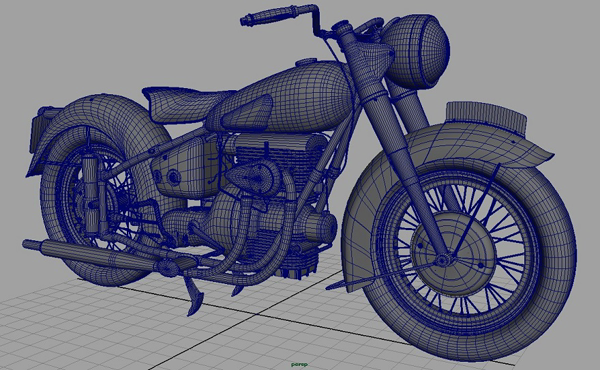
\includegraphics[width=0.5\textwidth,height=\textheight]{./images/wireframe_bike.png}
\caption{Model of Motorbike (\emph{seraphinacorazza.wordpress.com})}
\end{figure}

Modellers create pretty much all of the 3d assets (with the exception of 3d geometry created by FX TDs) required by a project. They have to meet not just artistic goals set by a combination of client notes and reference, but also technical specifications, some likely examples being:

\begin{itemize}
\tightlist
\item
  \emph{Correct and consistent detail level (or LOD for Level of Detail)}
\end{itemize}

\begin{quote}
Models will often be created with a number of LODS, so that the full detailed object doesn't always need to be rendered when it isn't required, for example when it is in the far distance of a shot. One workflow for creating these models is by starting from reference (or, if fortunate enough, a LIDAR scan) and, starting from a simple shape, building in progressively more detail so that the highest LOD is the last to be created.
\end{quote}

\begin{itemize}
\tightlist
\item
  \emph{Efficient UVs, so that the ratio between the UV space area and the 3D surface area is consistent throughout the model.}
\end{itemize}

\begin{quote}
Unless some parts of the model are more likely to have attention paid to than other parts. e.g.~character models, where faces often have higher resolution textures.
\end{quote}

\begin{itemize}
\tightlist
\item
  \emph{Efficient mesh topology, so its structure deforms well.}
\end{itemize}

\begin{quote}
This is very important in the games industry. They don't have the luxury of being able to sub-divide their meshes until they deform well, as the resource cost is exponentially expensive with each iteration.
\end{quote}

\hypertarget{types-of-modelling}{%
\paragraph{Types of Modelling}\label{types-of-modelling}}

Modelling is normally split into two categories: Hard surface and organic modelling.

Organic modelling encompasses anything with an irregular shape or something that is mathematically hard to express. Some examples include plants, poop and most characters \& animals. Sculpting is the preferred modelling method for organic modelling, which means using a program with specialised brushes that push, pull or otherwise deform parts of a model. ZBrush and Mudbox are both popular software packages that are used at studios.

Hard surface modelling is the skill of creating models that are \emph{not too difficult to express mathematically}*. But this does not in any way mean that they are any more difficult create than organic models. Hard surface modelling tasks include buildings, rigid props from bottles to mobile phones and most furniture. These shapes can be created using the more traditional and mathematical modelling tools, such as extruding and adding edge loops. Programs used to create these models include Autodesk Maya and SideFX Houdini.

These models are then passed off to texturing and rigging (if they are to be animated).

*\emph{Not an exact definition, but this was the result of reading lots of artists' individual opinions}

\hypertarget{rigging}{%
\subsubsection{Rigging}\label{rigging}}

\begin{figure}
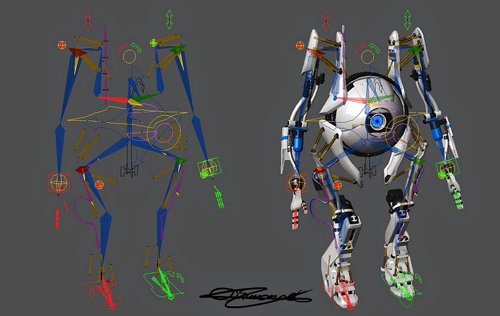
\includegraphics[width=0.5\textwidth,height=\textheight]{./images/portal_rig.png}
\caption{Portal Rig (\emph{James Ball})}
\end{figure}

A Rigger, sometimes called a Rigging TD, builds controllable rigs for models that require animation, such as vehicles and characters. For characters, this can involve building a skeleton which they bind to the mesh. Per-vertex weights are then painted for each skeletal bone, which defines how much influence that bone has on the vertex. These bones are normally hidden and more user-friendly controls are created.

It takes a lot of attention to detail and experience to make photorealistic, believable deformation. One challenge is the issue of volume preservation. With a skeleton of joints, as described above, even the most accurate painted weights will not maintain a consistent volume with the most complex animation, as the system has no concept of matter under the skin.

Riggers also work with muscle systems, which enable a more complex way of deforming an animal/living character. Shapes, defining individual muscles, are to be created and connected to the skeleton rig. This results in a more realistic definition in the skin and can help with volume preservation problem.

The most commonly used software package for this (in VFX) is Autodesk Maya, though other 3D packages, such as SideFX Houdini and Autodesk 3DSMax also have their own rigging systems.

\hypertarget{texture-shader-design}{%
\subsubsection{Texture \& Shader design}\label{texture-shader-design}}

\begin{figure}
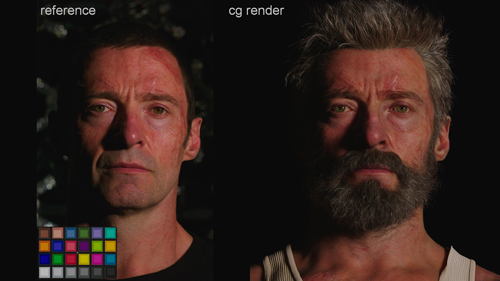
\includegraphics[width=0.5\textwidth,height=\textheight]{./images/logan_lookdev.png}
\caption{Logan Ref/Lookdev (\emph{Image Engine})}
\end{figure}

A texture artist designs the look of the surface of the model, by creating 2d maps, based on the model's UVs, that are ``wrapped around'' the model. These can be drawn digitally in a 2d program such as Adobe Photoshop, or artists can use more specialized texturing software such as Autodesk Mudbox and The Foundry's Mari, which provide lots of useful utilities which allow you paint directly on the model, and export textures afterwards*. This is advantageous as it means the texturer does not need to worry about issues related to making textures line up at seams (seams being the edges of separate UV shells that correspond to the same edge on the model).

\begin{figure}
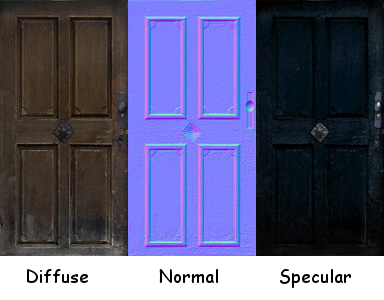
\includegraphics[width=0.5\textwidth,height=\textheight]{./images/door_texture_examples.png}
\caption{Door Texture Examples}
\end{figure}

Examples of maps that a texture artist might have to produce:

\hypertarget{diffuse-maps}{%
\paragraph{Diffuse Maps}\label{diffuse-maps}}

These maps show the colour light that an object reflects. Ideally, with no lighting effects baked in (such as reflections or specular highlights), these define the main colours of a model.

\hypertarget{bump-maps-or-height-maps}{%
\paragraph{Bump Maps (or Height maps)}\label{bump-maps-or-height-maps}}

Bump maps are generally monochrome maps which shows displacement of a texture perpendicular to the object. This is calculated by the value at a point of a bump map being multiplied by a constant, with a value of 0 being the most ``pushed-in'' point and 1 being the most ``sticky-outy'' (technical term). Though it is simply a lighting trick and adds no detail to the geometry.

\hypertarget{normal-maps}{%
\subparagraph{Normal Maps}\label{normal-maps}}

These bump maps can then be used in the process generate normal maps, a more accurate type of bump map. These are RGB maps that store the direction of the surface normals of a texture in a clever way. The R G \& B channels respectively correspond to the X Y and Z channels effectively giving you a 3D vector for each pixel of the UV map. These are then used to more realistically calculate the shading of a model.

\hypertarget{specular-maps}{%
\paragraph{Specular Maps}\label{specular-maps}}

These are RGB maps that define the ``shininess'' and specular colour of an object. The pixel intensity is proportional to the amount of light reflected from the point, and the RGB colour defines the colour of the reflection.

\hypertarget{displacement-maps}{%
\paragraph{Displacement Maps}\label{displacement-maps}}

As far as I can tell, these are identical to bump maps, in the way that they are monochrome maps that store perpendicular depth data. Though the difference is that displacement maps are actually used to deform the mesh, usually after being subdivided. I can only assume that these are used because working with super-high poly models is very computer-resource intensive, whereas working with 2d monochrome images isn't.

*\emph{I should mention that Photoshop had the ability for painting onto models for a number of years, but it's 2D compositing capabilities are more common and much stronger}

\hypertarget{step-3-shot-specific-work}{%
\subsection{Step 3: Shot Specific Work}\label{step-3-shot-specific-work}}

\hypertarget{matchmove}{%
\subsubsection{Matchmove}\label{matchmove}}

\begin{figure}
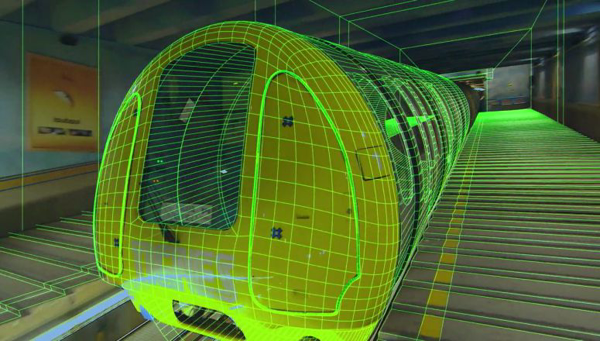
\includegraphics[width=0.5\textwidth,height=\textheight]{./images/matchmove.png}
\caption{Matchmove geometry over scan (\emph{QLBEANS})}
\end{figure}

Matchmoving is a massively important technique in visual effects which enables CG elements to have matching translation, rotation, and scale values to elements shot in the live-action scan. The most common way this is done is by individually tracking a number of 2D points in a scan, at different depths in real-world space, and by reconstructing a 3d camera a using complex math. This is the core of how the tracking system working in popular match moving software such as 3DEqualizer and PFTrack, though this system can sometimes struggle with footage that doesn't have many high-contrast, easy to track points. Another method, used in mocha Pro, that manages this issue quite well, is planar tracking, which aims to tracks whole surfaces, rather than individual points, though it doesn't work so well when there are no flat 2d planes, so there is no all-round best solution. Similar techniques to these can also be used to reconstruct 3D geometry and textures too.

Body tracking is another important match move task, which is the skill of matching a CG digi-double's animation to an actor in a live-action plate. This geometry can then be cached out and used later down the line by other departments, for example by lighting, if a full-CG replacement is required, or by FX if they need a simulation to react with the actor's body.

\hypertarget{animation}{%
\subsubsection{Animation}\label{animation}}

\begin{figure}
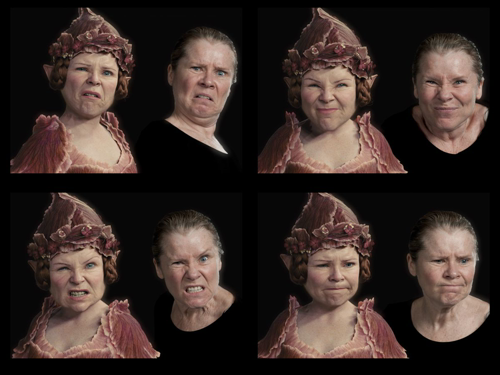
\includegraphics[width=0.6\textwidth,height=\textheight]{./images/anim_poses.png}
\caption{Animation Examples (\emph{Digital Domain})}
\end{figure}

3D animators make the characters passed down by modelling and rigged by rigging TDs come to life through keyframe animation, which is a technique I explain below. The goal of animators is to create a believable performance using a combination of reference and animation theory.

\hypertarget{keyframe-animation}{%
\paragraph{Keyframe Animation}\label{keyframe-animation}}

All rig controls will have at least some channels, possibly for controlling translation and/or rotation. These channels are then assigned certain values at specific frames, creating a keyframe. The channel's value between these keyframes are interpolated, either linearly or by using Bezier splines. These channels can be normally be edited by moving the handles in the viewport of your 3D program, or by manually editing the curves in the program's animation editor (sometimes called a graph editor), which will show you an interactive graphic visualisation of the animation curves.

\hypertarget{fx}{%
\subsubsection{FX}\label{fx}}

\begin{figure}
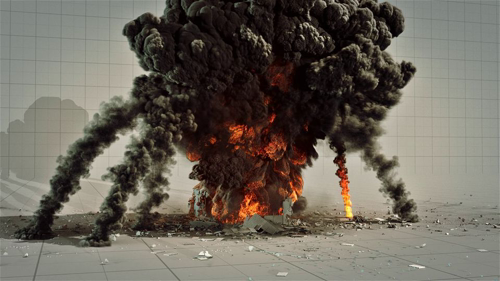
\includegraphics[width=0.5\textwidth,height=\textheight]{./images/fx.png}
\caption{Houdini FX Sim (\emph{Carlos Parmentier})}
\end{figure}

FX TDs (short for Effects Technical Directors) are responsible for using simulations in order to create creative 3D geometry caches which might model explosions, fire, destruction or fracturing shapes, or any other abstract or complex animation that doesn't easily fit into the role of other departments.

There is also another branch of FX, sometimes known as creature FX, who are responsible for using simulations upon the animated geometry of characters, in order to make them seem more real. The kind of tasks these artists might have to simulate could include character hair (also called a groom), skin \& muscles, and costumes.

There are always new simulation methods being published, and many well-known techniques are implemented and developed upon in software such as Autodesk Maya and SideFX Houdini.

\hypertarget{lighting}{%
\subsubsection{Lighting}\label{lighting}}

\begin{figure}
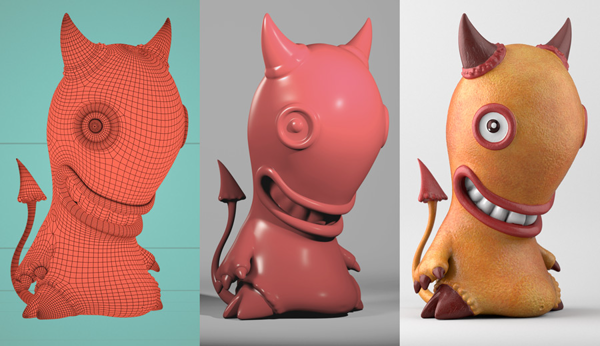
\includegraphics[width=0.5\textwidth,height=\textheight]{./images/lighting_before_after.png}
\caption{Lighting Before/After (\emph{Dylan Sisson})}
\end{figure}

A lighting TDs main role is to light 3D geometry in a way that matches another plate/scans lighting. This can be done either by using lots of different types of CG lights to create a rig, or also by using an HDRI (High Dynamic Range Image). HDRIs describe 360-degree images created by stitching together images of an environment taken from the same nodal point, at multiple exposure levels. This results in an image that ideally has data from all light sources from the darkest blacks to the brightest whites, with no clipping values, to realistically simulate the original environment's lighting conditions.

Another important responsibility of a lighting TD is to make sure there is consistency in the lighting in all of the elements in the shot. This sometimes means that the most physically realistic solution is not always the best.

Render configuration and efficiency, managing motion blur and noise, and writing/editing custom shaders might also be included in a lighting TD's responsibilities.

\hypertarget{step-4-2d}{%
\subsection{Step 4: 2D}\label{step-4-2d}}

\hypertarget{roto}{%
\subsubsection{Roto}\label{roto}}

\begin{figure}
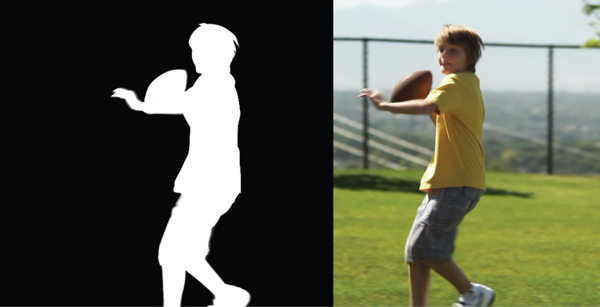
\includegraphics[width=0.5\textwidth,height=\textheight]{./images/roto_before_after.png}
\caption{Rotoscoping Example}
\end{figure}

Roto artists are responsible for creating alpha mattes from scans which isolate certain features. Ideally, a key would be easier and more efficient, but it is not always possible or practical to shoot in front of an evenly lit screen. The most common way this is done is by trying to break down the movement of the desired element in a way it can be defined by as few 2d spline-shapes as possible. Then these shapes are transformed and translated to follow the movement in the scan. Compositors can then take these elements and layer them over CG elements or combine them with other scans.

\hypertarget{preppaint}{%
\subsubsection{Prep/Paint}\label{preppaint}}

\begin{figure}
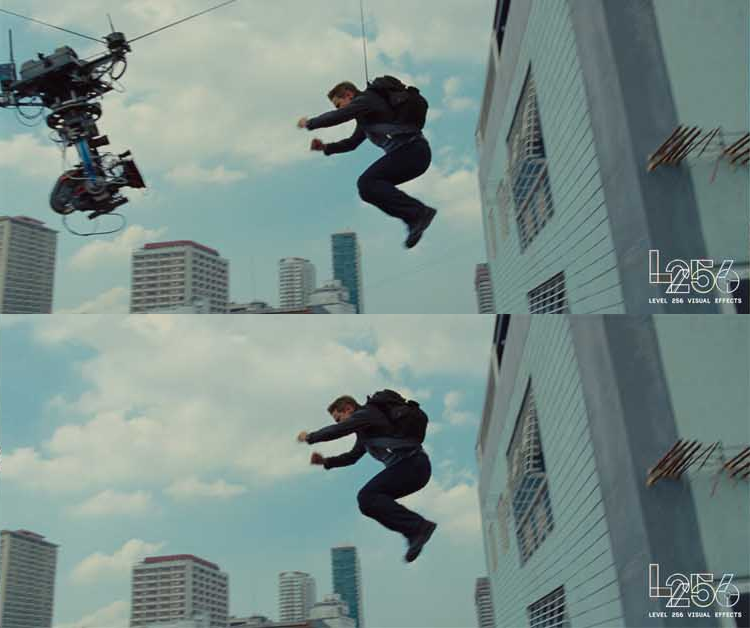
\includegraphics[width=0.5\textwidth,height=\textheight]{./images/prep_before_after.png}
\caption{Prep Before/After (\emph{Level 256 Visual Effects})}
\end{figure}

Prep has the job of cleaning up scans, ready for comp, mainly by painting. Painting, in the context of Prep, refers to the skill of believably reconstructing detail in a part of a scan that has been partially or completely occluded, by sampling from similar areas on the same or surrounding frames, or reference images. Some common paint removal tasks are required for:

\begin{itemize}
\tightlist
\item
  Dust shadows from footage shot on physical film.
\item
  Wires from actor harnesses.
\item
  Accidental or unavoidable boom poles, camera rigs and film crew members.
\item
  Items that conflict with latest creative decisions or that create continuity issues.
\end{itemize}

\hypertarget{comp}{%
\subsubsection{Comp}\label{comp}}

\begin{figure}

\includegraphics[width=0.5\textwidth,height=\textheight]{./images/mad_max_fx.png}
\caption{Mad Max Fury Road Composite (\emph{Iloura})}
\end{figure}

A comper's role is to combine the work of all of the earlier artists departments into a final shot. This involves combining any CG elements, DMP (Digital Matte Painting) work, prep elements and roto mattes with live action scans, in a way that looks believable enough to fool a viewer that it was shot once, through the lens of a single real camera.

An organised example of a Nuke node graph:

\begin{figure}
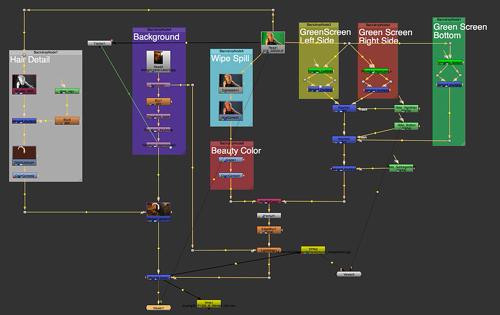
\includegraphics[width=0.5\textwidth,height=\textheight]{./images/nuke_node_graph.png}
\caption{Example Node Graph (\emph{jinguanghuang.com})}
\end{figure}

The most commonly used industry compositing software package is currently Nuke, which has been developed by The Foundry since 2007. It uses a node-based system, rather than the layer-based system found in compositing software such as the also very popular Adobe After Effects. One significant advantage of the node-based workflow is that it makes collaboration much easier. You can easily get an idea of what is happening in a well-organised nuke scene by zooming out and looking at the entire node graph, something that is much more difficult to do in a layer based system, especially when you are dealing with very large scene's (which is very likely in a VFX studio).

\pagebreak\hypertarget{linux}{%
\section{LINUX}\label{linux}}

Linux is an open source, UNIX-like operating system kernel designed to work on many different platforms. It has an active community developing it, so many distros (Linux distributions) are constantly evolving. It is impossible to count the available distros to try out, as people are free to modify existing source code and compile their own, though a quick search for ``Linux distros'' on \emph{DistroWatch}, a popular database of open source distros, returns over 800 results.

The most common distros are a particular flavour of Linux, called GNU/Linux, which is a combination of the Linux kernel and an assortment software from the GNU project, a collaborative development project with the goal to give people the freedom and encourage them to modify and share software. Richard Stallman, the founder of this project, wrote the first GNU General Public License (GPL) which enforces the aims of the project by requiring that any adaptations and redistributions are bound by the same license. Licenses with this ruling are given the name \emph{Copyleft}, as they impose restrictions which are protected by copyright law, but still allow for the modification and sharing of the work, something that is normally prohibited outside of ``fair use'' for most copyrighted material.

\hypertarget{open-source}{%
\subsubsection{Open Source}\label{open-source}}

Open source is a term used to describe software that has publicly available source code, meaning that developers/enthusiasts can modify and compile the package themselves. Software licensed under an open source license can usually be modified and redistributed by anyone who has acquired a copy of the software.

Here is the definition currently on the OSI's (Open Source Initiative) website:

\begin{quote}
Generally, open source software is software that can be freely accessed, used, changed, and shared (in modified or unmodified form) by anyone. Open source software is made by many people and distributed under licenses that comply with The Open Source Definition.
\end{quote}

Though Linux is not OSI licensed, it is licensed under GPL v2, a license written by the Free Software Foundation (FSF), an organisation also founded by Richard Stallman.

\hypertarget{using-linux}{%
\subsection{Using Linux}\label{using-linux}}

Linux is praised for having the ability to be incredibly lightweight, in the way that you can find fully-usable distributions that only use a minimal amount of space (\emph{Damn Small Linux (DSL) is a distro of only 50MB}) and in the sense that it doesn't have to consume a lot of computer resources. Some Linux distros don't even include a GUI (Graphical user interface) and are completely CLI-based (Command-line interface), which means that they are controlled entirely by typing text-based commands and writing scripts. Even for distros with a user-friendly graphical interface, in many cases, people find it easier to do certain tasks using commands, so terminal emulators exist in virtually every GUI-based distro so that you can still use the command-line interface. An example of a Linux installation using the MATE desktop environment is pictured below.

\begin{figure}
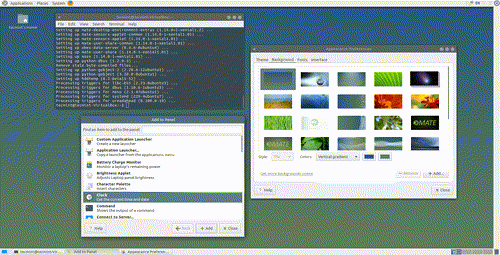
\includegraphics{./images/mate_desktop_example.png}
\caption{Linux running the MATE desktop environment}
\end{figure}

\hypertarget{useful-commands}{%
\subsubsection{Useful commands}\label{useful-commands}}

Here I won't explain everything that these commands can do as there is already enough documentation out there available to read. But I will cover the basic commands I use on a daily basis to get around Linux.

\hypertarget{cd}{%
\paragraph{cd}\label{cd}}

Changes the Current Working Directory (CWD) to the given path.

\hypertarget{ls}{%
\paragraph{ls}\label{ls}}

Lists files in the given path (or ./ by default). Using the \texttt{-a} argument also shows hidden files and the \texttt{-l} argument shows files in a list format. Other useful arguments include:

\begin{itemize}
\tightlist
\item
  \texttt{-h}: Shows human-readable file sizes (rather than displaying file sizes in bytes)
\item
  \texttt{-d}: Shows directories only
\item
  \texttt{-s}: Sorts files by filesize
\item
  \texttt{-R}: lists files recursively, meaning that it lists files that are contained in any subfolders of the directory.
\end{itemize}

For example:

\begin{verbatim}
~ >>> cd Downloads/
~/Downloads >>> ls
file1.txt  file2.mp4  my_book.epub
~/Downloads >>> ls -a
.  ..  .hidden_file  file1.txt  file2.mp4  my_book.epub
~/Downloads >>> ls -l
total 0
-rw-rw-r-- 1 sysadmin sysadmin 0 Mar  1 20:00 file1.txt
-rw-rw-r-- 1 sysadmin sysadmin 0 Mar  1 20:00 file2.mp4
-rw-rw-r-- 1 sysadmin sysadmin 0 Mar  1 20:00 my_book.epub
\end{verbatim}

\emph{Note: on Linux, \texttt{\textasciitilde{}} means your home directory, \texttt{.} is the current directory, and \texttt{..} refers to the parent directory}

\hypertarget{touch}{%
\paragraph{touch}\label{touch}}

Creates a new file with the given name.

\begin{verbatim}
~/Downloads >>> touch new_file.md
~/Downloads >>> ls
file1.txt  file2.mp4  my_book.epub  new_file.md
\end{verbatim}

\hypertarget{mkdir}{%
\paragraph{mkdir}\label{mkdir}}

Creates a directory, given a name and the desired path.

\begin{verbatim}
~/Downloads >>> cd ..
~ >>> ls
Desktop  Downloads
~ >>> mkdir ./my_folder
~ >>> ls
Desktop  Downloads  my_folder
\end{verbatim}

\hypertarget{cp}{%
\paragraph{cp}\label{cp}}

Copies a given file to the given destination. If you are copying a directory, you can use the \texttt{-r} flag to recursively copy the contents too.

\begin{verbatim}
~ >>> cp ./Downloads/new_file.md ./copied_file.md
~ >>> ls
Desktop  Downloads  my_folder  copied_file.md
\end{verbatim}

\hypertarget{mv}{%
\paragraph{mv}\label{mv}}

The same as cp but deletes the original file. You can technically use it to rename a file too.

\begin{verbatim}
~ >>> mv copied_file.md my_folder/moved_file.md
~ >>> ls
Desktop  Downloads  my_folder
~ >>> ls my_folder
moved_file.md
\end{verbatim}

\hypertarget{ln}{%
\paragraph{ln}\label{ln}}

This command is used to create file links, which are similar to what shortcuts are in the Windows OS. There are type types of links you can create with this command: Hard links (the default option) which all point to the same file on disk, whereas soft links (sometimes called symbolic links, created with the \texttt{-s} argument), effectively create a new file which is a pointer to the original file.

\begin{verbatim}
~ >>> ln  my_file.md ./Downloads -s
~ >>> ls -l /Downloads
-rw-rw-r-- 2 sysadmin sysadmin    0 Mar  6 20:50 my_file.md -> 
my_file.md
\end{verbatim}

\hypertarget{rm}{%
\paragraph{rm}\label{rm}}

Removes (deletes) a given file. The \texttt{-r} (recursive) flag can be used to remove directories.

\begin{verbatim}
~ >>> rm -r my_folder
~ >>> ls
Desktop  Downloads
\end{verbatim}

\hypertarget{alias}{%
\paragraph{alias}\label{alias}}

Assigns a given command/script to a given alias.

\begin{verbatim}
~ >>> alias m mkdir
~ >>> m my_new_folder
~ >>> ls
Desktop  Downloads  my_new_folder
\end{verbatim}

\hypertarget{tree}{%
\paragraph{tree}\label{tree}}

This script looks recursively through child folders and draws an easy to read folder structure diagram.


\pagebreak

\begin{verbatim}
~ >>> tree .
.
|-- Desktop
|-- Downloads
|   |-- file1.txt
|   |-- file2.mp4
|   `-- my_book.epub
`-- my_new_folder

3 directories, 3 files
\end{verbatim}

\hypertarget{find}{%
\paragraph{find}\label{find}}

Searches recursively from the given directory for a list of files that satisfy a given query, and can execute them all, given the \texttt{-exec} flag. One useful way to find files is by name. So by using the \texttt{-name} flag, you can pass the script a pattern to look for in the names of files. You can also find files by date, size, owner and many other attributes.

\begin{verbatim}
~ >>> find . -name "*book*"
./Downloads/my_book.epub
~ >>> find . -name "*b*"
./.bash_logout
./.bashrc
./Downloads/my_book.epub
\end{verbatim}

\hypertarget{cat}{%
\paragraph{cat}\label{cat}}

\texttt{cat}, short for concatenate, displays the contents of text files.

\begin{verbatim}
~ >>> cat Downloads/file1.txt
one two
three four
five six
seven eight
dog can
six elephants
lamp keyboard
\end{verbatim}

\hypertarget{grep}{%
\paragraph{grep}\label{grep}}

Returns a list of lines, given an input, that match a given pattern. It searches for lines inside given files, so in combination with find, you can easily search recursively for files containing specific strings, which can be very useful.


\pagebreak

\begin{verbatim}
~ >>> cat Downloads/file1.txt | grep six
five six
six elephants
~ >>> grep six Downloads/file1.txt
five six
six elephants
\end{verbatim}

\emph{Note: The pipe (\(\space\mid\space\)) character in the example above passes the output of the first command (\texttt{cat}) to the grep command}

\hypertarget{man}{%
\paragraph{man}\label{man}}

Opens up a documentation page for a given command. These pages are generally not \texttt{info} is a similar command included in the GNU project, which was intended to encourage a more long-form type of documentation. It has support for hyperlinks for referencing different chapters or files from within the docs. Many commands also have a \texttt{-h} or --help argument which shows you a quick summary of the main functions of the tool.

\hypertarget{compressingarchiving-files}{%
\subsection{Compressing/Archiving Files}\label{compressingarchiving-files}}

Inactive or old data, for example, logs or files from completed projects, can quickly build up on disks. So these files often need to compressed or archived, to free up some space for new data. I explained a little more about this in Unit 2.

\hypertarget{compression-on-linux}{%
\paragraph{Compression on Linux}\label{compression-on-linux}}

\texttt{gzip}, is a GNU tool for lossless file compression and decompression. Lossless refers to the type of compression that is used, which means that the original uncompressed file can be reproduced exactly from the compressed \texttt{gzip} (\texttt{gzip} is also the name of the file format). Lossy compression is when the some of the information from the original file is lost in the compression process, usually as the cost of further reducing the compressed file's size. This type of compression might not be completely suitable for plain text files, for obvious reasons, but is very useful for compressing image data, which, in many cases, doesn't need to be so precise.

How easy it is compress a file with \texttt{gzip}:

\begin{verbatim}
~ >>> ls
Desktop  Downloads  hasans_file.txt  my_folder
~ >>> gzip hasans_file.txt
~ >>> ls
Desktop  Downloads  hasans_file.txt.gz  my_folder
~ >>> gzip -l hasans_file.txt.gz
         compressed        uncompressed  ratio uncompressed_name
               5632               47044  88.1% hasans_file.txt
\end{verbatim}

And we can uncompress it just as easily, by using the \texttt{gunzip} (g- unzip) command:

\begin{verbatim}
~ >>> gunzip hasans_file.txt.gz
~ >>> ls
Desktop  Downloads  hasans_file.txt  my_folder
\end{verbatim}

Linux also comes with another compression tool, called \texttt{bzip2}, which is used in the same way as \texttt{gzip}, but uses more complex algorithms, meaning that it can take a little longer to compress/uncompress data, but can also reduce it to a smaller size than is possible with \texttt{gzip}. \texttt{bunzip2} works in the same way as \texttt{gunzip} for uncompressing files. The conventional file extensions for files compressed with \texttt{bzip2} are \texttt{.bz} and \texttt{.bz2}.

\hypertarget{archival}{%
\paragraph{Archival}\label{archival}}

Archives combine multiple individual files into one single file. This could be useful if you wanted to compress this data together, as you would only have to compress this one file, which, depending on the algorithms used, might even be more time efficient than compressing them separately. The standard UNIX utility for this is \texttt{tar} (short for tape-archive). In Linux, there is a GNU rewrite which replaces this, also called \texttt{tar}.

You can use tar to create, extract and browse tar files (sometimes called tarballs). To create a tar file, you have to use the \texttt{-c} argument to enable create ``mode'' and the \texttt{-f} argument to tell it to write to a given filename.

Here I create a new archive containing my text files:

\begin{verbatim}
~/my_folder >>> ls
hasans_file.txt    hasans_file_2.txt  hasans_file_4.txt
hasans_file_1.txt  hasans_file_3.txt  hasans_file_5.txt
~/my_folder >>> tar -cf my_archive.tar ./*
~/my_folder >>> ls -lh
total 568K
-rw-rw-r-- 1 sysadmin sysadmin  46K Mar  2 18:28 hasans_file.txt
-rw-rw-r-- 1 sysadmin sysadmin  46K Mar  2 19:02 hasans_file_1.txt
-rw-rw-r-- 1 sysadmin sysadmin  46K Mar  2 19:03 hasans_file_2.txt
-rw-rw-r-- 1 sysadmin sysadmin  46K Mar  2 19:03 hasans_file_3.txt
-rw-rw-r-- 1 sysadmin sysadmin  46K Mar  2 19:03 hasans_file_4.txt
-rw-rw-r-- 1 sysadmin sysadmin  46K Mar  2 19:03 hasans_file_5.txt
-rw-rw-r-- 1 sysadmin sysadmin 280K Mar  2 19:32 my_archive.tar
\end{verbatim}

You can see here that the archive is equal (roughly) to the sum of the files it was created from's individual sizes. This is because this archive is completely uncompressed. We could use the \texttt{gzip} command if we wanted to compress it, or we could use \texttt{tar}'s \texttt{-z} flag, which creates a gzip-compressed tar archive. The \texttt{-j} argument exists for \texttt{bzip2} compression too. The convention for compressed individual files is to append the \texttt{.gz}/\texttt{.bz} file extension to the end of the file. Let me show you an example:


\pagebreak

\begin{verbatim}
~/my_folder >>> tar -czf my_archive.tar.gz ./*
~/my_folder >>> ls -lh my_archive.tar.gz
-rw-rw-r-- 1 sysadmin sysadmin 8.2K Mar  2 19:49 my_archive.tar.gz
\end{verbatim}

This created a vastly smaller filer as a result. The \texttt{gzip}-compressed tar is 34 times smaller than the original, the only tradeoff is that you have to uncompress it before you can read it, which is not a major issue if these are files aren't expecting much use. You can uncompress and read them with the \texttt{tar} command too, with the \texttt{-t} flag to enable ``browse files'' mode and the \texttt{-z} flag again to uncompress the data first with \texttt{gunzip}:

\begin{verbatim}
~/my_folder >>> tar -tzf my_archive.tar.gz
./hasans_file.txt
./hasans_file_1.txt
./hasans_file_2.txt
./hasans_file_3.txt
./hasans_file_4.txt
./hasans_file_5.txt
\end{verbatim}

\hypertarget{security-1}{%
\subsection{Security}\label{security-1}}

Linux adopts UNIX's ``Everything is a file'' feature, meaning that data from devices and peripherals such as printers, keyboards, disk drives and networked machines are all accessible via the file system. This is done by using virtual filesystems which are all mounted so that they are visible as one file hierarchy.

\hypertarget{usersgroups}{%
\paragraph{Users/Groups}\label{usersgroups}}

User and group permissions are used to control access in Linux. To create a new user, you can use the \texttt{useradd} and \texttt{passwd} commands:

\begin{verbatim}
~ >>> useradd hasan -d /home/hasan
\end{verbatim}

The \texttt{-d} flag sets the home (\texttt{\textasciitilde{}}) directory.

\begin{verbatim}
~ >>> passwd hasan
Enter new UNIX password:
Retype new UNIX password:
passwd: password updated successfully
\end{verbatim}

Creating new groups and adding a user to them is just as simple, using the \texttt{groupadd} and \texttt{usermod} commands:

\begin{verbatim}
~ >>> useradd
~ >>> groupadd gods
~ >>> groupadd kings
~ >>> usermod -G gods,kings hasan
\end{verbatim}

And, finally, we can see what groups a user is assigned to by using the \texttt{id} command.

\begin{verbatim}
~ >>> id hasan
uid=1002(hasan) gid=0(root) groups=1002(gods),1003(kings)
\end{verbatim}

The default user, \texttt{root}, automatically has access to every file, with no regard for permissions.

\hypertarget{file-permissions}{%
\paragraph{File Permissions}\label{file-permissions}}

Every file in Linux file system has its own properties, one of which being its own permission levels, which is used to restrict access to certain files and directories. There are three types of access you can to a file: read, write and execute. An easy way to see a file's attributes is to use the command \texttt{ls\ -l}:

\begin{verbatim}
~ >>> ls -lh
-rw-r--r-- 1 root root 2.3K Mar  5 20:49 hasans_medical_records.csv
\end{verbatim}

\begin{figure}
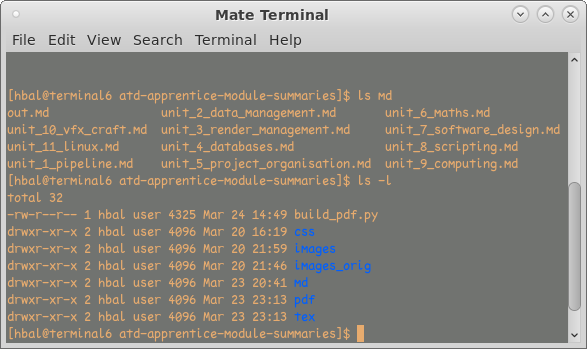
\includegraphics[width=0.7\textwidth,height=\textheight]{./images/terminal_environment.png}
\caption{\texttt{ls\ -l} command in a terminal.}
\end{figure}

Here we can see multiple columns each with different data about the file. In order, these columns describe, in this order:

\begin{itemize}
\tightlist
\item
  Filetype + Permission level.
\item
  The number of hard links pointing to file.
\item
  File's owner.
\item
  File's group.
\item
  File size.
\item
  Last edit: date and time.
\end{itemize}

The file type + permission level is not immediately intuitive, so I will explain what it means. The first character dictates the type of file that this is. In most cases, this will be either \texttt{-}, for standard files, \texttt{d} for directories and \texttt{l} for links. The second part is made up of nine permission bits, with 3 bits controlling read, write and execute access for the file owner, group and other users.

There are two common ways for these permissions to be written. One, as you can see in the \texttt{ls} examples above, is to use \texttt{r}, \texttt{w} and \texttt{x} (read, write and execute) in place of their respective bits to show that the access that has been granted, and \texttt{-} in place of bits that are not enabled. With this example, a file with \texttt{rwxr-\/-r-\/-} has read, write and execute access for the owner, but anyone else will only have read access. Another way to write these permissions would be to use a number in place of each set of 3 bits (\texttt{rwx}). 111, in binary, is equal to 7 in denary, so we can use the digits 0-7 to represent every possible \texttt{rwx} combination. With this logic, 220 would equal \texttt{-w-\/-w-\/-\/-\/-} and 775 would equal \texttt{rwxrwxr-x}.

The \texttt{chmod} command can be used to modify a files permissions if you happen to have write access to the file. The 0-7 digit method is the easiest method to use with this command.

\begin{verbatim}
~ >>> chmod 000
~ >>> ls -l
---------- 1 root root 2.3K Mar  5 20:49 hasans_medical_records.csv
~ >>> chmod 777
~ >>> ls -l
-rwxrwxrwx 1 root root 2.3K Mar  5 20:49 hasans_medical_records.csv
\end{verbatim}
